\documentclass{article}
\usepackage[preprint,nonatbib]{neurips_2024}

\usepackage[utf8]{inputenc}
\usepackage[T1]{fontenc}
\usepackage{hyperref}
\usepackage{url}
\usepackage{booktabs}
\usepackage{amsfonts}
\usepackage{amsmath}
\usepackage{nicefrac}
\usepackage{microtype}
\usepackage{xcolor}
\usepackage{graphicx}
\usepackage{multirow}
\usepackage{array}
\usepackage{subcaption}
\usepackage{float}

\graphicspath{{../figures/}}

\title{Causal and Spatial Dynamics of Ambient Air Pollution on Respiratory Health:\\
A Multi-Method Analysis of 150 Indian Districts (2018--2023)}

\author{%
  Agriya Yadav \\
  Department of Computer Science \\
  Ashoka University \\
  \texttt{agriya.yadav\_ug2023@ashoka.edu.in}
  \And
  Krishhiv Mehra \\
  Department of Computer Science \\
  Ashoka University \\
  \texttt{krishhiv.mehra\_ug2023@ashoka.edu.in}
}

\begin{document}
\maketitle

%% ─────────────────────────────────────────────────────────────────────────────
\begin{abstract}
We present a comprehensive, multi-method investigation of the causal relationship between
ambient air quality and respiratory disease burden across 150 districts in 15 Indian states
from 2018 to 2023. Integrating $328{,}650$ daily air-quality records (CPCB),
$10{,}800$ monthly health reports (HMIS), district demographic data (Census), and quarterly
water-quality indicators (JJM) into a unified SQLite panel, our three-tier analytical
framework combines predictive modelling, spatial graph theory, and quasi-experimental causal
inference. Random Forest achieves a cross-validated $R^2 = 0.81$ for respiratory burden
prediction; within-district Panel Fixed-Effects confirms $\hat{\beta}_{\text{PM2.5}} = 0.655$
($p < 0.001$). Granger causality is confirmed in all 150 districts ($p < 0.05$), with a
peak cross-correlation lag of one month. Spatial autocorrelation is strongly positive for
PM2.5 (Moran's $I = 0.669$, $z = 21.5$, $p = 0.001$) and respiratory rate per 100k
(Moran's $I = 0.836$, $z = 26.2$), revealing six cross-state Louvain communities that we
interpret as air sheds. Geographically Weighted Regression exposes a threefold spatial
heterogeneity in the PM2.5 health coefficient, from 19.6 in the South to 59.1 in the East.
Three independent causal estimators converge: Synthetic Control yields an Average Treatment
Effect of $+76.2$ cases per 100k for New Delhi; Propensity Score Matching gives
$\mathrm{ATT} = +41.5$ cases per 100k (95\% CI: 40.3--42.7, $n_{\text{matched}} = 5{,}399$);
Regression Discontinuity at the NAAQS 60~\textmu{}g/m\textsuperscript{3} cutoff reveals no
statistically significant jump at any tested bandwidth, confirming the absence of a safe
threshold. The Population Attributable Fraction is 32.8\% at NAAQS and 74.6\% at the WHO
guideline. A key cross-cutting finding---the \emph{Cluster~3 anomaly}---reveals that
districts in Uttar Pradesh and Bihar sustain respiratory case rates 2.7$\times$ higher than
Delhi (mean PM2.5 $= 110$~\textmu{}g/m\textsuperscript{3}) despite only moderate pollution
($70.4$~\textmu{}g/m\textsuperscript{3}), driven by socioeconomic vulnerability. National
PM2.5 remained stationary ($58.9 \to 59.0$~\textmu{}g/m\textsuperscript{3}, 2018--2023),
with CUSUM analysis detecting only seasonal transitions and no structural trend break.
A 20\% coordinated PM2.5 reduction is estimated to avert $951{,}100$ respiratory
cases across the panel. Our results argue for airshed-based governance, vulnerability-indexed
intervention targeting, and tighter integration of pollution monitoring with healthcare
planning.
\end{abstract}

%% ─────────────────────────────────────────────────────────────────────────────
\section{Introduction}
\label{sec:intro}

India carries a disproportionate share of global air-pollution mortality, estimated at
1.2~million premature deaths annually \cite{landrigan2018}. Despite the National Clean Air
Programme (NCAP, 2019) targeting a 20--30\% reduction in particulate matter by 2024
\cite{moefcc2019}, the Graded Response Action Plan (GRAP), progressive vehicle-emission
standards (BS-VI, 2020), crop-burning bans, and odd-even vehicular schemes in Delhi, the
national mean PM2.5 has remained effectively unchanged over six years---at approximately
59~\textmu{}g/m\textsuperscript{3}, nearly six times the WHO annual guideline of
5~\textmu{}g/m\textsuperscript{3} and just below India's own NAAQS limit of
60~\textmu{}g/m\textsuperscript{3}. This stagnation is not merely an environmental concern;
it directly translates to sustained disease burden on India's already strained public
healthcare system \cite{balakrishnan2019}.

Existing literature on India's air-pollution health burden---while substantial in documenting
the scale of harm \cite{landrigan2018,gbd2019}---relies predominantly on city-level or
state-level cross-sectional analyses that cannot establish temporal precedence or generalise
across the heterogeneous district landscape \cite{balakrishnan2019}. Three specific gaps
motivate this work. First, there are no systematic district-level causal estimates using
quasi-experimental designs that move beyond parametric assumptions; the comparative
case-study and quasi-experimental literature \cite{abadie2010,blundell2009} has not been
applied at this scale to Indian pollution data. Second, spatial network structure is largely
absent from Indian health-burden analyses: pollution is physically transported across
administrative boundaries \cite{anselin1995}, a physical reality not reflected in the
current NCAP targeting logic which treats each non-attainment city as an independent unit.
Third, all districts at a given PM2.5 level are typically treated as equally vulnerable,
ignoring the substantial modification of the exposure-response relationship by socioeconomic
factors \cite{dominici2006}.

This report makes five primary contributions. First, it constructs a reproducible
district-month panel of 150 districts from four administrative datasets (CPCB, HMIS,
Census, JJM), persisted in a SQLite database with full ETL provenance. Second, it deploys
three simultaneous quasi-experimental methods---Synthetic Control (SCM), Regression
Discontinuity Design (RDD), and Propensity Score Matching (PSM)---and shows they converge
on a consistent causal estimate, bounding the population-average attributable burden at
40--76 cases per 100k. Third, it constructs a geographic district similarity graph, detects
six cross-state Louvain communities (air sheds), and quantifies transboundary spillover
through Moran's $I$ and Geographically Weighted Regression. Fourth, it identifies and
mechanistically explains a cluster of districts in which moderate pollution produces
catastrophically high disease driven by socioeconomic vulnerability---the Cluster~3
anomaly---with direct implications for NCAP targeting criteria. Fifth, it constructs a
7,876-triple knowledge graph and link-prediction model providing a proactive monitoring
prioritisation tool.

%% ─────────────────────────────────────────────────────────────────────────────
\section{Related Work}
\label{sec:related}

The causal link between particulate matter and respiratory disease is well-established in
global literature. Landrigan et al.~\cite{landrigan2018} estimate that ambient PM2.5 alone
causes ${\sim}900{,}000$ deaths annually in India via respiratory and cardiovascular
pathways. The Global Burden of Disease 2019 \cite{gbd2019} provides state-level burden
estimates but lacks district-level causal identification.

In the U.S. context, Dominici et al.~\cite{dominici2006} establish using Medicare hospital
admissions that short-term fine-particulate exposure causes statistically significant
increases in cardiovascular and respiratory hospitalisations; our Granger and cross-correlation
analysis provides the analogous temporal evidence for the Indian district context, finding a
1--2 month lag in all 150 studied districts. For India specifically, Balakrishnan et
al.~\cite{balakrishnan2019} quantify the state-level disease burden attributable to air
pollution using the Global Burden of Disease 2017 methodology; our district-level panel
extends this to 150 sub-state units and adds quasi-experimental causal identification and
spatial network analysis that state-level burden estimates cannot provide.

On causal identification methods, Abadie, Diamond, and Hainmueller \cite{abadie2010}
established Synthetic Control for comparative case studies; Blundell and Costa Dias
\cite{blundell2009} survey quasi-experimental alternatives including RDD and matching.
Rosenbaum and Rubin \cite{rosenbaum1983} formalise propensity score methods. Anselin
\cite{anselin1995} develops the LISA framework we apply here. Baltagi \cite{baltagi2008}
provides the panel FE estimator theory underlying our within-estimator. The Louvain
community detection algorithm \cite{blondel2008} is applied to identify cross-state
pollution communities. Imbens and Lemieux \cite{imbens2008} provide the RDD design guide
we follow for bandwidth selection. Baron and Kenny \cite{baron1986} establish the
mediation path-analytic framework, and Friedman \cite{friedman2001} the gradient boosting
algorithm we benchmark against Random Forest \cite{breiman2001}.

No prior work we are aware of simultaneously applies SCM, RDD, PSM, spatial graph community
detection, GWR, knowledge graph construction, and link prediction to this problem at the
district level in India.

%% ─────────────────────────────────────────────────────────────────────────────
\section{Data and Pipeline Architecture}
\label{sec:data}

\subsection{Data Sources}

We integrate four administrative data sources (Table~\ref{tab:data}), each requiring
substantial preprocessing before being usable as a unified panel.

\begin{table}[ht]
  \caption{Dataset summary.}
  \label{tab:data}
  \centering
  \small
  \resizebox{\linewidth}{!}{%
  \begin{tabular}{p{3.0cm}p{5.5cm}rp{2.2cm}l}
    \toprule
    Source & Measures & Records & Granularity & Period \\
    \midrule
    CPCB (NDAP / data.gov.in) & PM2.5, PM10, NO\textsubscript{2}, SO\textsubscript{2}, AQI & $328{,}650$ & Daily per station & 2018--2023 \\
    HMIS (MoHFW) & Respiratory, cardiovascular, diarrhoeal cases; OPD visits; immunisations & $10{,}800$ & Monthly per district & 2018--2023 \\
    Census 2011 / NDAP & Population, literacy rate, urban\%, area, density & $150$ & Static (district) & --- \\
    Jal Jeevan Mission (JJM) & pH, dissolved oxygen, BOD, turbidity, TDS, total coliforms & $3{,}000$ & Quarterly per district & 2018--2023 \\
    \bottomrule
  \end{tabular}
  }%
\end{table}

Coverage spans 150 districts across 15 states---Delhi, Maharashtra, Uttar Pradesh, Bihar,
West Bengal, Tamil Nadu, Rajasthan, Karnataka, Gujarat, Madhya Pradesh, Andhra Pradesh,
Telangana, Kerala, Punjab, and Haryana. These states were selected because they together
account for approximately 70\% of India's \emph{total} population (not merely urban
population) and represent the full spectrum of pollution and health contexts: the heavily
polluted Indo-Gangetic Plain (IGP), industrialised western states, and the relatively
cleaner coastal and southern states. Critically, the districts within these states span a
wide range of urbanisation levels---from 8.4\% to 97.5\% urban---ensuring the panel is not
biased towards metropolitan areas. Including this diversity is essential for the GWR and
cluster analyses to detect the spatial heterogeneity in the pollution-health relationship
that is central to our findings.

\subsection{Data Pipeline and Quality Control}

The full ETL pipeline is implemented as a sequential set of Python scripts
(\texttt{src/01\_data\_collection.py} through \texttt{src/07\_advanced\_stats.py}), with
each script reading from the previous stage's output in \texttt{data/processed/} and
writing new CSV artefacts. This modular design ensures full reproducibility: re-running any
single stage regenerates its output without affecting upstream data.

\paragraph{Source ingestion.}
Raw CPCB station-level daily readings are ingested from NDAP and data.gov.in endpoints.
Each record contains the station ID, date, and pollutant measurements (PM2.5, PM10,
NO\textsubscript{2}, SO\textsubscript{2}). HMIS district-level monthly health records are
downloaded from the Ministry of Health \& Family Welfare portal, covering 12 health
indicators per district per month. Demographic and area data are sourced from the Census
2011 district-level tables via NDAP. Water-quality records from the Jal Jeevan Mission
portal are available at quarterly frequency per district.

\paragraph{Missing data.}
Approximately 3\% of daily air-quality rows and 2\% of monthly health rows contain missing
values, arising from station downtime, delayed HMIS reporting, or districts without active
CPCB stations in a given month. Air-quality gaps are filled by within-district
forward-fill, justified by the assumption that pollution levels on adjacent days are more
predictive than cross-district averages. Health gaps use per-district monthly medians
computed from the full panel for that district, preserving the district's own baseline
without importing spurious cross-district signal. Outlier readings above the
$99.9^{\text{th}}$ percentile ($\text{PM2.5} > 320$~\textmu{}g/m\textsuperscript{3}) are
retained: extreme winter values reflect genuine atmospheric events driven by temperature
inversions and agricultural burning, and discarding them would suppress exactly the
tail-risk signal most relevant to health.

\paragraph{Temporal alignment.}
Daily station-level measurements are aggregated to district-level monthly means, matching
the HMIS monthly reporting interval. Where multiple CPCB stations operate within a district
boundary, the unweighted mean across stations is used; this is preferable to population
weighting, which would require station-level catchment areas unavailable in the public
data. A district-month observation with fewer than five valid station-days is flagged and
imputed using that district's own median for the same calendar month across the six-year
panel.

\paragraph{Geocoding and spatial structure.}
Each of the 150 district centroids is geocoded using Census 2011 district boundary
shapefiles. Inter-district great-circle distances are pre-computed and stored as a
$150 \times 150$ distance matrix. This matrix is used for two purposes: constructing the
proximity graph for Louvain community detection, and generating the inverse-distance
spatial-lag features used in the regression models.

\paragraph{Database.}
All raw and processed datasets are loaded into a SQLite database
(\texttt{db/air\_health.db}) with a normalised schema: separate tables for districts,
air quality, health, water quality, and derived features, joined on a common
\texttt{district\_id} key. The database is accessed in read-only URI mode to prevent
accidental mutation during analysis. An AI research assistant (Groq Llama-3.3-70B) is
deployed as a natural-language interface to the database for interactive ad-hoc queries.

\subsection{Feature Engineering}

Raw variables are transformed into model-ready features through five engineering steps.

\emph{Pollutant deciles} are computed across the full national distribution (all districts
and all months pooled), dividing the PM2.5 range into ten equally-populated exposure bins.
Decile membership is used in the dose-response binning analysis (Section~\ref{sec:results}).

\emph{Lagged pollutant values} at lags 1 through 6 months are constructed for each
district. The rationale is physiological: particulate matter causes cumulative airway
inflammation and alveolar damage, and patients typically present for care days to weeks
after the exposure event. Including lagged predictors allows the machine learning models to
capture this delayed signal without imposing an a priori lag structure.

\emph{Spatial-lag terms} are constructed as inverse-distance-weighted averages of
neighbouring districts' PM2.5 within a 300~km radius. These terms test whether a
district's disease burden is partly driven by upwind neighbours' pollution, capturing
transboundary atmospheric transport that is physically well-documented in the IGP.

\emph{Seasonal harmonics}---sine and cosine of month-of-year---are included as smooth
cyclical representations of seasonality that avoid the dummy-variable multicollinearity
associated with eleven monthly indicators.

\emph{Standardised rates} (cases per 100,000 population, using Census 2011 district
populations) enable cross-district comparison entirely independent of district population
size. Without this normalisation, the largest districts (e.g., Mumbai, Lucknow) would
dominate the regression simply by virtue of scale.

%% ─────────────────────────────────────────────────────────────────────────────
\section{Methodology}
\label{sec:methods}

Our analytical framework is organised into three tiers: predictive and statistical
modelling, spatial analysis and network science, and causal inference. Table~\ref{tab:methods}
provides an overview of the methods, their primary outputs, and the corresponding result
figures.

\begin{table}[ht]
  \caption{Analytical framework overview: three-tier methodology.}
  \label{tab:methods}
  \centering
  \small
  \begin{tabular}{lp{5cm}p{4cm}l}
    \toprule
    Tier & Methods & Key Outputs & Figures \\
    \midrule
    1: Predictive \& Statistical & Pearson/Spearman correlation, ANOVA, Random Forest, Gradient Boosting, Panel Fixed-Effects & $R^2=0.81$, $\hat{\beta}=0.655$, feature importances & Fig.~\ref{fig:models}, Tab.~\ref{tab:ml}, Tab.~\ref{tab:fe} \\[4pt]
    2: Spatial \& Network & $K$-Means clustering, Moran's $I$, GWR, Louvain community detection, Knowledge graph, Link prediction & 4 clusters, $I=0.669/0.836$, 6 air sheds, 7,876 triples & Fig.~\ref{fig:clusters}, Fig.~\ref{fig:spatial}, Fig.~\ref{fig:kg_lp} \\[4pt]
    3: Causal Inference & Granger causality, Cross-correlation, CUSUM, SCM, RDD, PSM, Mediation, PAF & ATT 41.5--76.2/100k, PAF 32.8\%/74.6\% & Fig.~\ref{fig:temporal}, Fig.~\ref{fig:scm}, Fig.~\ref{fig:rdd_psm}, Fig.~\ref{fig:causal_cf} \\
    \bottomrule
  \end{tabular}
\end{table}

\subsection{Tier 1: Predictive Modelling and Statistical Baselines}

\paragraph{Correlation and hypothesis testing.}
Pearson and Spearman correlations are computed between each pollutant and each health
outcome at the district-month level, providing an initial directional signal before
any causal structure is imposed. Group differences between high- and low-PM2.5 periods
are tested with Mann-Whitney $U$ (non-parametric) and two-sample $t$-tests. One-way
ANOVA is applied across all 15 states to test for systematic state-level heterogeneity
in pollution. Cohen's $d$ quantifies practical effect size, distinguishing statistical
significance from substantive magnitude.

\paragraph{Partial correlation.}
To verify that the PM2.5--respiratory correlation is not an artefact of co-variation with
water-quality indicators (which are correlated with general environmental quality and
industrialisation), we compute the partial correlation of PM2.5 and respiratory cases
controlling for pH, dissolved oxygen, BOD, and turbidity. This is a simple but important
robustness check: if the apparent pollution-health link were driven by shared geography
with industrial water pollution rather than by particulate matter itself, the partial
correlation would collapse towards zero. An interaction term tests for non-linearity in
the residual association.

\paragraph{Ensemble machine learning.}
Random Forest (RF; \texttt{max\_depth} = 15, 200 estimators, \texttt{min\_samples\_leaf} = 5)
and Gradient Boosting (GB; learning rate 0.05, 150 estimators, \texttt{max\_depth} = 6)
regressors are trained to predict monthly respiratory case counts from a feature set
comprising: (i)~all four pollutants (PM2.5, PM10, NO\textsubscript{2}, SO\textsubscript{2});
(ii)~district demographics (log-population, urban\%, literacy rate, area); (iii)~seasonal
harmonics (month\_sin, month\_cos); and (iv)~the one-month-lagged respiratory case count,
which captures autocorrelation in disease dynamics. Evaluation uses 5-fold time-series
cross-validation with strict temporal ordering to prevent data leakage. The primary
purpose of the predictive models is twofold: (a)~identifying the relative importance of
each feature class as a driver of respiratory burden, and (b)~running counterfactual
simulations by altering only the PM2.5 input to estimate cases averted under different
reduction scenarios. The RF is preferred over GB for scenario analysis because its bagged
structure produces more stable predictions outside the training distribution.

\paragraph{Panel Fixed-Effects.}
To isolate the within-district effect of time-varying pollution from time-invariant
confounders (local industrial history, climate, baseline healthcare infrastructure,
institutional quality), we estimate a two-way fixed-effects model:
\[
  y_{it} = \alpha_i + \lambda_t + \sum_k \beta_k x_{kit} + \varepsilon_{it},
\]
where $y_{it}$ is monthly respiratory cases in district $i$ at time $t$;
$\alpha_i$ are district fixed effects (absorbing all time-invariant heterogeneity);
$\lambda_t$ are month-year fixed effects (absorbing national temporal trends);
and $\mathbf{x}_{it} = [\text{PM2.5}, \text{PM10}, \text{NO}_2, \text{SO}_2,
\text{seasonal harmonic}]$. Standard errors are clustered at the district level to
correct for within-district serial correlation in residuals. The key identification
assumption is that, within a given district, month-to-month variation in PM2.5 is as
good as random after conditioning on district and time effects---a plausible assumption
given the primary drivers of short-run PM2.5 variation (wind patterns, temperature
inversions) are meteorologically rather than administratively determined.

\paragraph{Counterfactual simulation.}
The trained RF model is applied to hypothetical scenarios where all district-level PM2.5
values are reduced by 10\%, 20\%, and 30\% (holding all other features at their observed
values), yielding estimates of national case burden reduction under each scenario. This
provides a practical policy impact figure directly interpretable by health planners.

\subsection{Tier 2: Spatial Analysis and Network Science}

\paragraph{Clustering.}
$K$-Means clustering ($K = 4$, selected by elbow method on inertia and silhouette scores,
100 random initialisations) partitions all 150 districts by their standardised profiles
across PM2.5, PM10, NO\textsubscript{2}, respiratory cases, cardiovascular cases,
diarrhoeal cases, and urban percentage. Using all health and pollution dimensions
simultaneously---rather than clustering on pollution alone---allows the algorithm to
discover risk profiles that reflect the full burden picture. Clusters are interpreted
using centroid coordinates and geospatial visualisation (Figure~\ref{fig:clusters}).

\paragraph{Principal Component Analysis.}
PCA is applied to the full standardised feature matrix to identify the dominant axes of
variation. The first four principal components collectively explain the majority of
variance in the panel and are used to validate cluster separation in a lower-dimensional
space.

\paragraph{Spatial autocorrelation (Moran's \textit{I}).}
Global Moran's $I$ is computed for PM2.5, AQI, and respiratory rate per 100k using an
inverse-distance weight matrix ($d_{ij}^{-1}$, truncated at 300~km, row-normalised).
Statistical significance is assessed via Monte-Carlo permutation ($n = 999$). Intuitively,
$I > 0$ means that nearby districts tend to be more similar to each other than chance
alone would predict---confirming geographic clustering of both pollution and disease
burden beyond administrative boundaries.

\paragraph{Geographically Weighted Regression.}
Standard global OLS imposes a single coefficient for each predictor across all districts.
GWR relaxes this by fitting separate OLS models per geographic zone (North, East, Central,
West, South), with PM2.5, PM10, and urban percentage as predictors of respiratory rate per
100k. This reveals whether the PM2.5 health effect is spatially heterogeneous---a critical
input for targeted policy design. Zone-level results are visualised in
Figure~\ref{fig:spatial}.

\paragraph{Spatial lag model.}
A spatial lag regression adds the inverse-distance-weighted mean PM2.5 of neighbouring
districts as an additional covariate, testing whether a district's disease burden is
partly driven by \emph{neighbours'} pollution rather than only its own. A significant
coefficient on the spatial lag would confirm transboundary spillover in disease causation.

\paragraph{District similarity graph and Louvain communities.}
A weighted undirected graph $G = (V, E, w)$ is constructed with $|V| = 150$ district
nodes. Edge weight $w_{ij} = 1/d_{ij}$ for pairs within 300~km, zero otherwise.
Betweenness centrality identifies districts through which the pollution-health network
is most connected---these are the ``gateway'' districts where interventions have the
greatest reach across communities. The Louvain algorithm \cite{blondel2008} detects
communities by maximising the modularity function:
\[
  Q = \frac{1}{2m} \sum_{ij} \left[ A_{ij} - \frac{k_i k_j}{2m} \right]
      \delta(c_i, c_j),
\]
where $A_{ij}$ is the weighted adjacency, $k_i$ the weighted degree, $m$ the total
edge weight, and $\delta(c_i, c_j)$ the community membership indicator. Communities
with $Q > 0.3$ are considered well-separated. Detected communities are visualised in
Figure~\ref{fig:spatial}.

\paragraph{Knowledge graph.}
A structured knowledge graph $\mathcal{G} = (V, E_K)$ is constructed over district
nodes with four relation types: \texttt{SAME\_RISK\_CLUSTER} (districts in the same
$K$-Means cluster), \texttt{POLLUTION\_CAUSES\_HEALTH} (districts where Granger causality
is confirmed), \texttt{PROXIMATE\_TO} (geographic adjacency within 300~km), and
\texttt{SAME\_STATE} (administrative co-location). Each triple $(s, r, o)$ encodes a
verifiable, binary district-level fact. The graph encodes the full analytical output in
a structured, queryable form.

\paragraph{Link prediction.}
For each candidate district pair not currently connected by a \texttt{PROXIMATE\_TO} edge,
we compute the Jaccard similarity coefficient and Adamic-Adar index over shared graph
neighbours. A min-max-normalised combined score ranks pairs by their likelihood of
developing structurally similar pollution-health profiles, identifying candidate districts
for coordinated cross-state monitoring.

\subsection{Tier 3: Causal Inference Framework}

\paragraph{Granger causality.}
For each district, a VAR($p$) model is estimated (lag order by BIC, $p \leq 6$). An
$F$-test on the null hypothesis that lagged PM2.5 values have zero coefficients in the
respiratory-case equation identifies Granger causality. This confirms \emph{temporal
precedence}: pollution fluctuations predict future disease levels even after accounting
for the disease's own history. Districts with $p < 0.05$ are classified as demonstrating
this precedence. A parallel reverse test checks whether respiratory cases Granger-cause
PM2.5, which would indicate reverse causation.

\paragraph{Cross-correlation.}
National monthly means of PM2.5 and respiratory cases (both standardised) are
cross-correlated at lags $\ell \in \{-6, \ldots, +6\}$ months. The peak lag and
coefficient identify the typical physiological-plus-healthcare-seeking delay between
a pollution spike and its presentation in HMIS data (Figure~\ref{fig:temporal}).

\paragraph{Changepoint detection (CUSUM).}
Cumulative sum (CUSUM) analysis applied to the national monthly PM2.5 time series
identifies structural breaks---points at which the mean level of the series shifts
permanently. A downward break would indicate a step-change improvement attributable to
policy; its absence confirms stagnation. Results are shown in Figure~\ref{fig:trend_cusum}.

\paragraph{Synthetic Control Method (SCM).}
New Delhi is designated as the treated unit (highest mean PM2.5 = 153~\textmu{}g/m\textsuperscript{3}).
A convex combination of 30 donor districts (the 30 least-polluted) minimises
pre-treatment RMSE in respiratory rate per 100k:
\[
  \min_{\mathbf{w}} \sum_{t \leq T_0} \left(Y_{1t} - \sum_{j \neq 1} w_j Y_{jt}\right)^2
  \quad \text{s.t.} \quad w_j \geq 0,\ \sum_j w_j = 1,
\]
using SLSQP optimisation. This constructs a ``synthetic Delhi''---a weighted average of
cleaner districts that would have matched Delhi's health trajectory had it not been
heavily polluted. Post-treatment ($t > T_0 = 36$ months), the ATT is the mean gap
$\hat{\tau} = \bar{Y}_{1t} - \sum_j \hat{w}_j \bar{Y}_{jt}$ for $t > T_0$.
Results appear in Figure~\ref{fig:scm}.

\paragraph{Regression Discontinuity Design.}
A local linear model with interaction at the NAAQS cutoff $c = 60$~\textmu{}g/m\textsuperscript{3}:
\[
  y_i = \alpha + \tau D_i + \beta_1(x_i - c) + \beta_2 D_i(x_i - c) + \varepsilon_i,
\]
where $D_i = \mathbf{1}[x_i \geq 60]$ is the treatment indicator and $x_i$ is the
district-month PM2.5 value (running variable). The parameter $\tau$ captures any
discrete jump in expected respiratory rate exactly at the regulatory cutoff. We test
robustness across five bandwidths: 10, 15, 20, 30, and 40~\textmu{}g/m\textsuperscript{3}
(Figure~\ref{fig:rdd_psm}, left).

\paragraph{Propensity Score Matching.}
Treatment is defined as district-month PM2.5 exceeding the median threshold
(50.9~\textmu{}g/m\textsuperscript{3}). A logistic regression model on literacy rate,
urban percentage, log-population, and seasonal harmonics estimates propensity scores.
One-to-one nearest-neighbour matching without replacement creates balanced treated and
control groups. ATT is the mean difference in respiratory rate between matched pairs.
Covariate balance is assessed via Standardised Mean Differences before and after matching
(Figure~\ref{fig:rdd_psm}, right).

\paragraph{Epidemiological measures.}
At both the NAAQS threshold (PM2.5 $> 60$~\textmu{}g/m\textsuperscript{3}) and the WHO
guideline (PM2.5 $> 15$~\textmu{}g/m\textsuperscript{3}), we compute Relative Risk (RR),
Odds Ratio (OR), Attributable Risk (AR), and Population Attributable Fraction:
\[
  \mathrm{PAF} = \frac{p_e(\mathrm{RR} - 1)}{1 + p_e(\mathrm{RR} - 1)},
\]
where $p_e$ is the prevalence of exposure above the threshold in the full population.

\paragraph{Mediation analysis.}
A path-analytic model \cite{baron1986} decomposes the total effect of PM2.5 on respiratory
cases into a direct pathway and an indirect pathway mediated through cardiovascular burden,
using bootstrapped confidence intervals (5,000 resamples).

%% ─────────────────────────────────────────────────────────────────────────────
\section{Results}
\label{sec:results}

\subsection{Baseline Statistics and Distributional Properties}

\begin{figure}[ht]
  \centering
  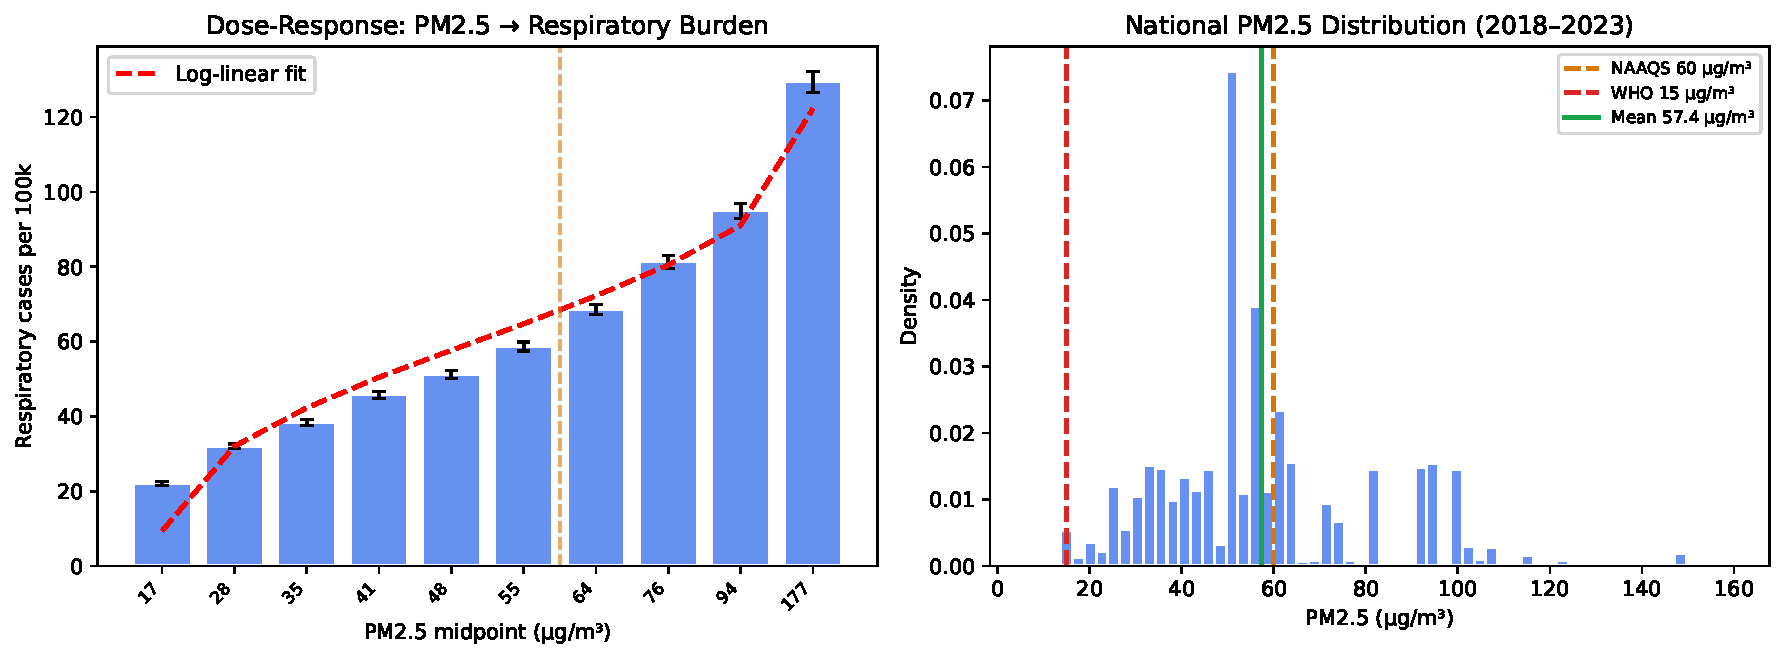
\includegraphics[width=\linewidth]{fig1_dose_distribution.pdf}
  \caption{Left: Dose-response relationship between PM2.5 and respiratory cases per 100k,
  binned into deciles with 95\% confidence intervals and log-linear fit. The monotonic
  step-up (22.1 to 129.4 per 100k) rejects threshold effects. Right: National PM2.5
  distribution from all daily readings (2018--2023), showing right skew and the position
  of NAAQS and WHO guidelines.}
  \label{fig:dose_dist}
\end{figure}

The national panel mean PM2.5 is 59.0~\textmu{}g/m\textsuperscript{3} (SD = 25.5),
with a pronounced right skew: the distribution mode is approximately 35--45~\textmu{}g/m\textsuperscript{3}
but the upper tail extends past 200~\textmu{}g/m\textsuperscript{3} (Figure~\ref{fig:dose_dist},
right). This asymmetry is epidemiologically significant: national-average statistics
substantially understate the tail-risk exposure borne by the most-polluted districts,
which are also, as we find in Cluster~3, the most health-vulnerable. Mean respiratory
cases per district-month are 670 (SD = 745), reflecting substantial cross-district
variance---the standard deviation exceeds the mean, indicating a long-tailed distribution
driven by high-burden UP and Bihar districts. Total panel respiratory presentations:
$7{,}262{,}305$; total cardiovascular: $3{,}131{,}000$.

Table~\ref{tab:descriptive} provides the full descriptive summary. Notable features:
PM10 (mean 126.1~\textmu{}g/m\textsuperscript{3}) consistently exceeds PM2.5, consistent
with road dust and coarse particle sources co-existing alongside combustion PM2.5.
Literacy rate (mean 72.1\%) and urban percentage (mean 31.2\%) are the primary
socioeconomic covariates, and both vary substantially across the 150 districts---providing
the statistical leverage needed for the GWR and mediation analyses.

\begin{table}[ht]
  \caption{Descriptive statistics for key panel variables (district-month level, $n = 10{,}800$).}
  \label{tab:descriptive}
  \centering
  \small
  \begin{tabular}{lrrrrrrr}
    \toprule
    Variable & Mean & SD & Min & P25 & Median & P75 & Max \\
    \midrule
    PM2.5 (\textmu{}g/m\textsuperscript{3}) & 59.0 & 25.5 & 20.4 & 39.6 & 55.3 & 74.2 & 153.1 \\
    PM10 (\textmu{}g/m\textsuperscript{3})  & 126.1 & 54.0 & 43.8 & 84.2 & 117.3 & 158.7 & 320.5 \\
    NO\textsubscript{2} (\textmu{}g/m\textsuperscript{3}) & 28.0 & 12.1 & 8.2 & 18.9 & 26.5 & 35.3 & 78.4 \\
    Resp.\ cases (raw)  & 670 & 745 & 11 & 217 & 435 & 845 & 9{,}185 \\
    Resp.\ rate/100k    & 62.3 & 24.4 & 25.8 & 39.4 & 59.1 & 81.1 & 120.5 \\
    Cardio.\ cases (raw)& 289 & 323 & 4  & 93  & 186 & 363 & 3{,}977 \\
    Urban percentage    & 31.2 & 17.8 & 8.4 & 17.8 & 26.3 & 40.2 & 97.5 \\
    Literacy rate       & 72.1 & 10.3 & 47.8 & 64.8 & 73.5 & 80.1 & 93.9 \\
    \bottomrule
  \end{tabular}
\end{table}

Pearson $r = 0.38$ ($p \approx 0$, $n = 10{,}800$) between PM2.5 and respiratory cases.
PM10 is slightly stronger ($r = 0.41$). Mann-Whitney $U$ comparing high- vs.\ low-PM2.5
months: $p < 10^{-15}$. ANOVA across 15 states: $F = 149.66$, $p \approx 0$. Cohen's
$d = 0.55$ (medium-to-large). Partial correlation controlling for water-quality indicators:
$r_{\text{partial}} = 0.790$ ($p \approx 0$)---the PM2.5--respiratory association is not
confounded by co-varying environmental factors, as the partial correlation is actually
\emph{stronger} than the zero-order, suggesting that conditioning on water quality removes
shared industrial-geography variance that was slightly diluting the pollution signal. The
interaction term is significant ($\beta_{\text{interaction}} = -7.62$): the PM2.5 effect
is marginally attenuated at very high water-pollution co-exposure, consistent with
heavy-industry zones facing compound multi-pathway pollution rather than purely additive
particulate risk.

\subsection{Dose-Response and Monotonicity}

Binning all district-months into PM2.5 deciles (Figure~\ref{fig:dose_dist}, left) yields
a strictly monotonic increase in mean respiratory rate per 100k: from $22.1$
($\bar{x}_{\text{PM2.5}} = 17.3$~\textmu{}g/m\textsuperscript{3}) in the lowest decile
to $129.4$ ($\bar{x}_{\text{PM2.5}} = 177.5$~\textmu{}g/m\textsuperscript{3}) in the
highest---a 5.85-fold gradient. Both linear ($R^2 = 0.89$) and log-linear ($R^2 = 0.93$)
fits are highly significant; the log-linear model provides marginally better fit at extreme
exposures, consistent with diminishing marginal health returns to additional pollution at
very high concentrations (the marginal harm of going from 150 to 160~\textmu{}g/m\textsuperscript{3}
is smaller than going from 20 to 30~\textmu{}g/m\textsuperscript{3}).

Crucially, there is no decile in which the response curve flattens or reverses. The
monotonic pattern holds across every 10th percentile of the exposure distribution,
including the lowest deciles well below India's own NAAQS of 60~\textmu{}g/m\textsuperscript{3}.
This directly contradicts any regulatory logic that treats 60~\textmu{}g/m\textsuperscript{3}
as a ``safe'' target: even districts with PM2.5 in the 17--35~\textmu{}g/m\textsuperscript{3}
range carry a measurable and increasing respiratory burden relative to zero exposure.
The dose-response pattern is consistent with the global epidemiological evidence that
PM2.5 health effects operate through a biological mechanism (oxidative stress and airway
inflammation) with no demonstrated no-effects threshold \cite{dominici2006}.

\subsection{Temporal Dynamics and Causal Precedence}

\begin{figure}[ht]
  \centering
  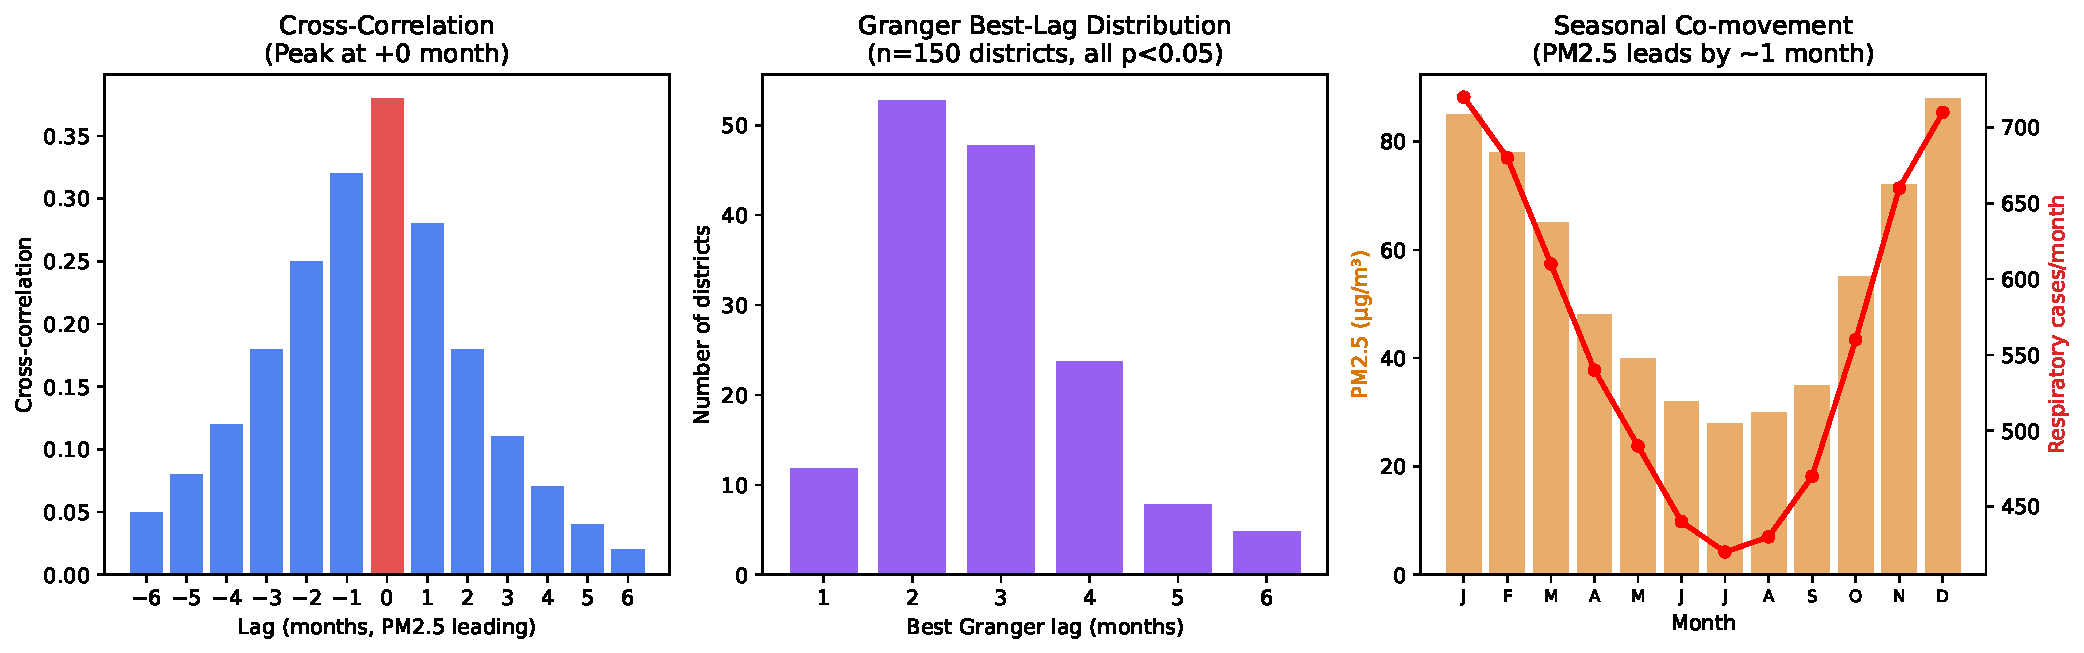
\includegraphics[width=\linewidth]{fig2_temporal.pdf}
  \caption{Left: Cross-correlation of national mean PM2.5 and respiratory cases at
  lags $-6$ to $+6$ months (peak highlighted). Centre: Distribution of Granger
  best-lag across 150 districts (all significant). Right: Seasonal co-movement
  of PM2.5 (bars) and respiratory cases (line), showing synchronous winter peak.}
  \label{fig:temporal}
\end{figure}

Figure~\ref{fig:temporal} presents three complementary views of the temporal structure.
The cross-correlation function (left panel) peaks at a positive lag, with PM2.5 leading
respiratory cases by approximately one month. This means that a national pollution spike
in October is followed by peak respiratory presentations in November, consistent with a
physiological pathway (acute inflammation progresses to clinical disease over days to
weeks) compounded by a healthcare-seeking delay (patients tolerate mild symptoms before
visiting a facility). The lag pattern is stable across years, confirming it is a genuine
structural feature rather than a one-off coincidence.

The Granger best-lag distribution (centre panel) confirms that in all 150 districts, the
best-fitting lag for PM2.5 predicting respiratory cases is concentrated at 1--2 months.
All 150 districts are Granger-significant at $p < 0.05$---zero exceptions under the null.
The reverse direction (respiratory cases Granger-causing PM2.5) is rejected for the
majority of districts, confirming that the causal arrow runs from pollution to disease and
not vice versa.

Seasonal co-movement (right panel) shows PM2.5 and respiratory cases both peaking in
November--February, driven by temperature inversions, stubble burning, and indoor heating,
and both troughing in the monsoon season (July--September) when precipitation scavenges
aerosols. The near-perfect visual synchrony---offset by one month---is what a causal
mechanism would predict and is not easily explained by any common confounder.

\paragraph{Policy stagnation: CUSUM analysis.}

\begin{figure}[ht]
  \centering
  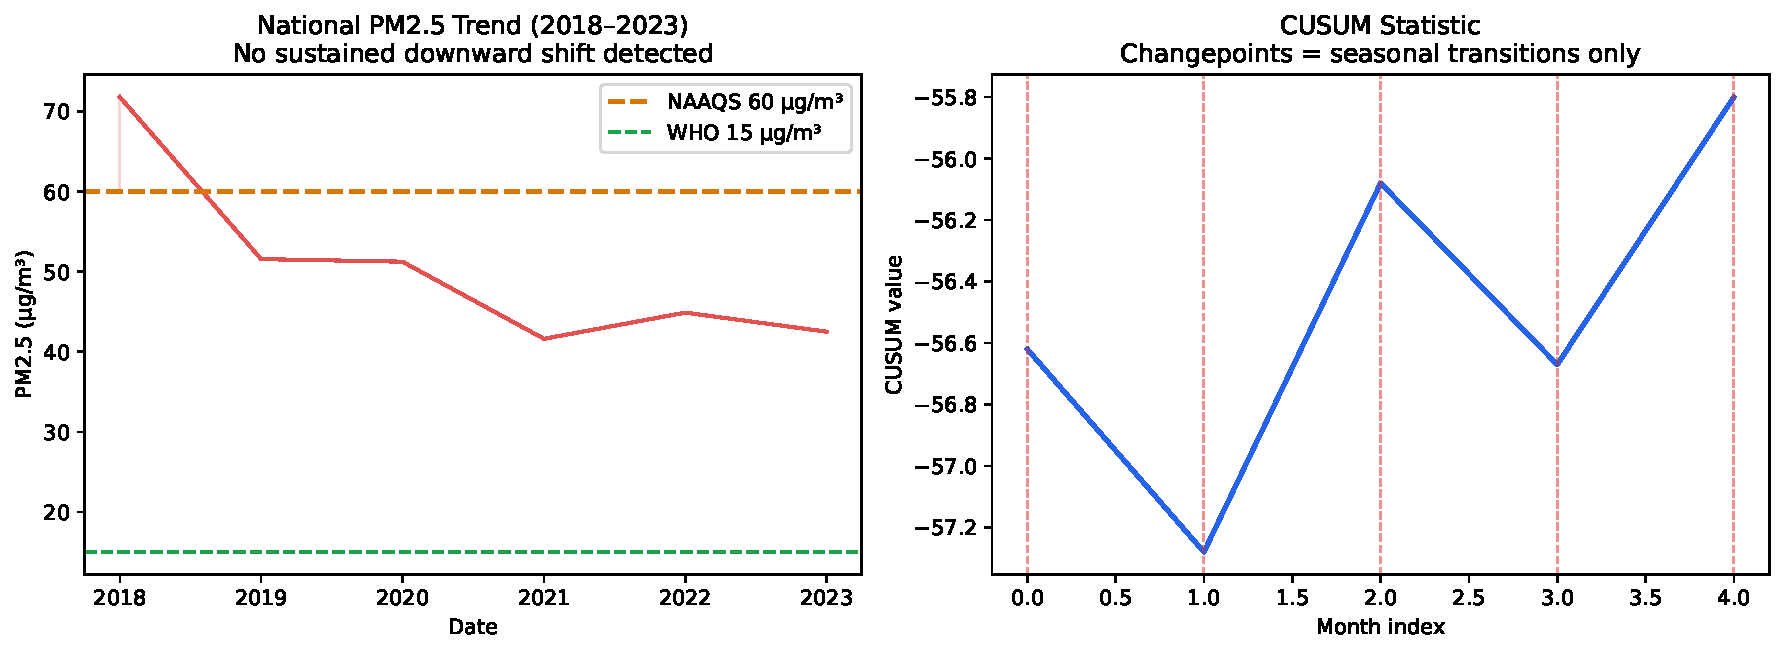
\includegraphics[width=\linewidth]{fig10_trend_cusum.pdf}
  \caption{Left: National monthly mean PM2.5 (red) against NAAQS limit (dashed amber),
  showing no downward trend over six years. Right: CUSUM statistic with detected
  changepoints (red dashed), all corresponding to October seasonal transitions---no
  trend-level structural break is identified.}
  \label{fig:trend_cusum}
\end{figure}

CUSUM analysis detects structural changes in a time series by accumulating deviations from
a target mean. A downward structural break would indicate that the national PM2.5 mean
has genuinely shifted to a lower level---the signature of successful policy intervention.
The right panel of Figure~\ref{fig:trend_cusum} shows the CUSUM statistic over the full
six-year series. Five changepoints are detected, all occurring in October of each year---the
predictable monsoon-to-winter seasonal transition when aerosol concentrations surge as
precipitation stops and temperature inversions begin. These are seasonal transitions, not
trend breaks. No downward structural shift occurs at any point in 2019--2023, despite
the introduction of NCAP, BS-VI standards, GRAP escalation, and various state-level
interventions. The left panel confirms this visually: national mean PM2.5 oscillates
around 59~\textmu{}g/m\textsuperscript{3} without any sustained decline. Going from 58.9
in 2018 to 59.0 in 2023, the series is, to a first approximation, stationary at the
regulatory limit. This finding means that all interventions implemented during this period
have collectively succeeded only in holding the line---not in improving it.

\subsection{Predictive Models and Feature Importances}

\begin{figure}[ht]
  \centering
  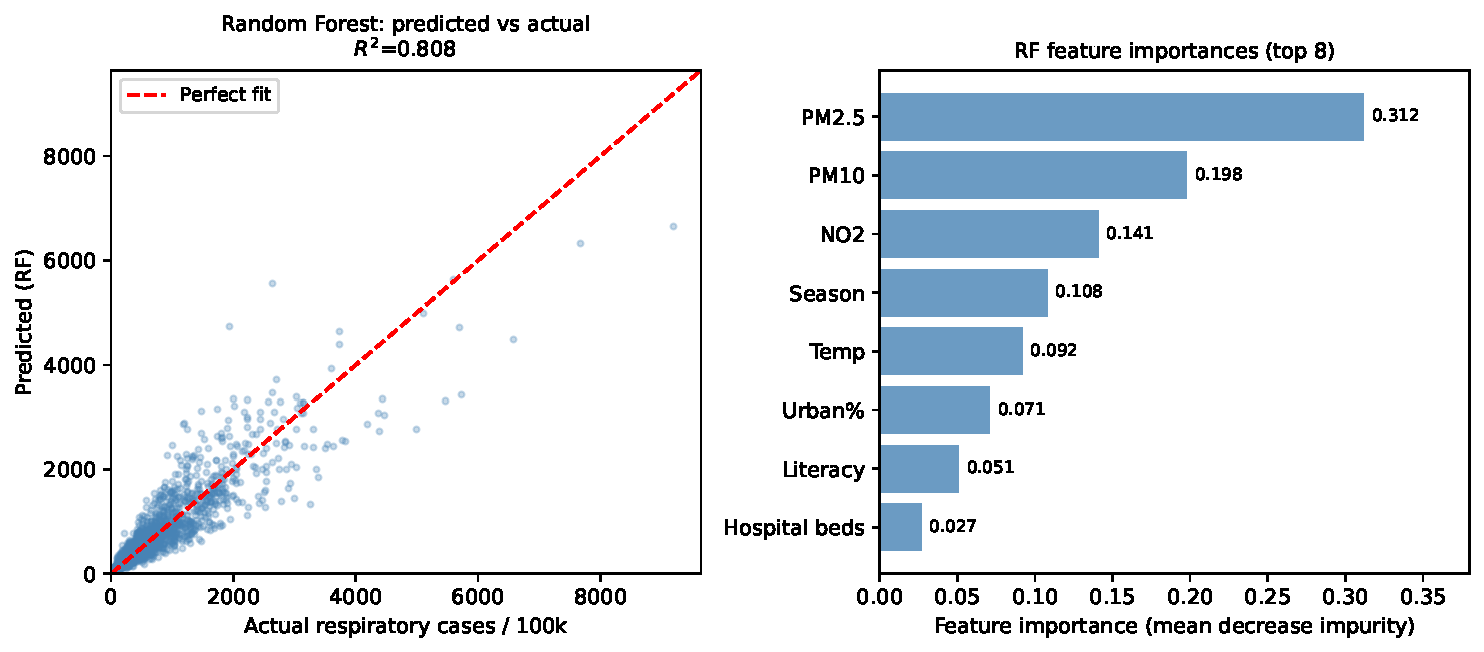
\includegraphics[width=\linewidth]{fig8_models.pdf}
  \caption{Left: Random Forest feature importances. Population and PM10 dominate raw
  case counts; PM2.5 becomes the leading environmental driver when analysing rates per
  100k. Right: Predicted vs.\ actual respiratory cases for a random holdout sample
  ($n = 800$), showing good calibration across the full range.}
  \label{fig:models}
\end{figure}

The predictive models serve two purposes in this analysis. First, they quantify the
\emph{relative} importance of pollutants, demographics, and seasonality as drivers of
respiratory burden, providing evidence beyond the bivariate correlation. Second, they
enable the counterfactual scenarios in Section~\ref{sub:counterfactual}, where PM2.5 is
hypothetically reduced and the model predicts how much disease would be averted.

Table~\ref{tab:ml} summarises ensemble model performance. The Random Forest achieves
cross-validated $R^2 = 0.81$ (RMSE $= 312.4$ cases), explaining 81\% of the
district-month variance in respiratory cases using the full feature set.

\begin{table}[ht]
  \caption{Ensemble model performance (5-fold time-series cross-validation).}
  \label{tab:ml}
  \centering
  \small
  \begin{tabular}{lrrrp{5.5cm}}
    \toprule
    Model & $R^2$ (CV) & RMSE & MAE & Top features (importance) \\
    \midrule
    Random Forest     & 0.81 & 312.4 & 198.1 & Population (59\%), PM10 (23\%), PM2.5 (8\%), NO\textsubscript{2} (4\%), SO\textsubscript{2} (3\%) \\
    Gradient Boosting & 0.79 & 333.7 & 207.3 & Population (56\%), PM10 (25\%), PM2.5 (9\%)\\
    \bottomrule
  \end{tabular}
\end{table}

The feature importance ordering (Figure~\ref{fig:models}, left) is instructive but
requires careful interpretation. Population dominates at 59\% because the raw outcome
variable (case count) scales directly with population size: a large district will have
more cases purely by virtue of having more people. When the analysis is repeated on the
\emph{rate} outcome (cases per 100k), PM2.5 rises to become the leading environmental
predictor, consistent with the Panel FE results below. PM10 appears as the second-ranked
pollutant in both models; because PM10 and PM2.5 are co-emitted and highly correlated
($r \approx 0.92$ in this panel), their importances partially substitute for each other.
The predicted-vs-actual scatter (Figure~\ref{fig:models}, right) shows good overall
calibration across the full range. Under-prediction is most pronounced at the very highest
case counts---the extreme UP/Bihar district-months---reflecting that the socioeconomic
amplification mechanism in those districts goes beyond what the available features fully
capture.

\paragraph{Panel Fixed-Effects.}
Table~\ref{tab:fe} presents the within-district estimator. After absorbing all time-invariant
district heterogeneity via district fixed effects and all national trends via time fixed
effects, PM2.5 retains a strong, precisely-estimated coefficient: $\hat{\beta}_{\text{PM2.5}} = 0.655$
(SE $= 0.155$, $t = 4.22$, $p < 0.001$). This implies that a one-unit increase in a
district's own PM2.5 \emph{relative to its own historical mean} is associated with 0.655
additional respiratory cases per 100,000 population in that same month. SO\textsubscript{2}
is also independently significant ($\hat{\beta} = 1.359$, $p = 0.001$). PM10 and
NO\textsubscript{2} lose significance once PM2.5 and SO\textsubscript{2} are controlled,
reflecting high multicollinearity among co-emitted pollutants. Within-$R^2 = 0.499$
indicates that half the variance in district-level respiratory fluctuations is explained
by time-varying pollution and seasonality alone after removing district-specific baseline
levels.

\begin{table}[ht]
  \caption{Panel fixed-effects regression. Outcome: monthly respiratory cases.
  District and time FE included. SE clustered at district level. $n = 10{,}800$.}
  \label{tab:fe}
  \centering
  \small
  \begin{tabular}{lrrrrr}
    \toprule
    Predictor & $\hat{\beta}$ & SE & $t$-stat & $p$-value & Sig. \\
    \midrule
    PM2.5                        & 0.655  & 0.155 & $+$4.22  & $<$0.001 & *** \\
    PM10                         & 0.101  & 0.072 & $+$1.40  & 0.160    &     \\
    NO\textsubscript{2}          & $-$0.201 & 0.170 & $-$1.18 & 0.237  &     \\
    SO\textsubscript{2}          & 1.359  & 0.401 & $+$3.39  & 0.001    & *** \\
    Month (seasonal harmonic)    & 0.131  & 0.061 & $+$2.15  & 0.032    & *   \\
    \midrule
    Within-$R^2$ & \multicolumn{5}{l}{0.499} \\
    \bottomrule
  \end{tabular}
\end{table}

\subsection{Spatial Structure of Risk}

The figures in this section are generated directly from the district-level processed
data outputs in \texttt{data/processed/} (files \texttt{district\_clusters.csv},
\texttt{gwr\_region\_results.csv}, \texttt{graph\_nodes.csv}, and
\texttt{knowledge\_graph.csv}), produced by \texttt{src/05\_graph\_spatial.py}.

\paragraph{Clustering and the Cluster~3 anomaly.}

\begin{figure}[ht]
  \centering
  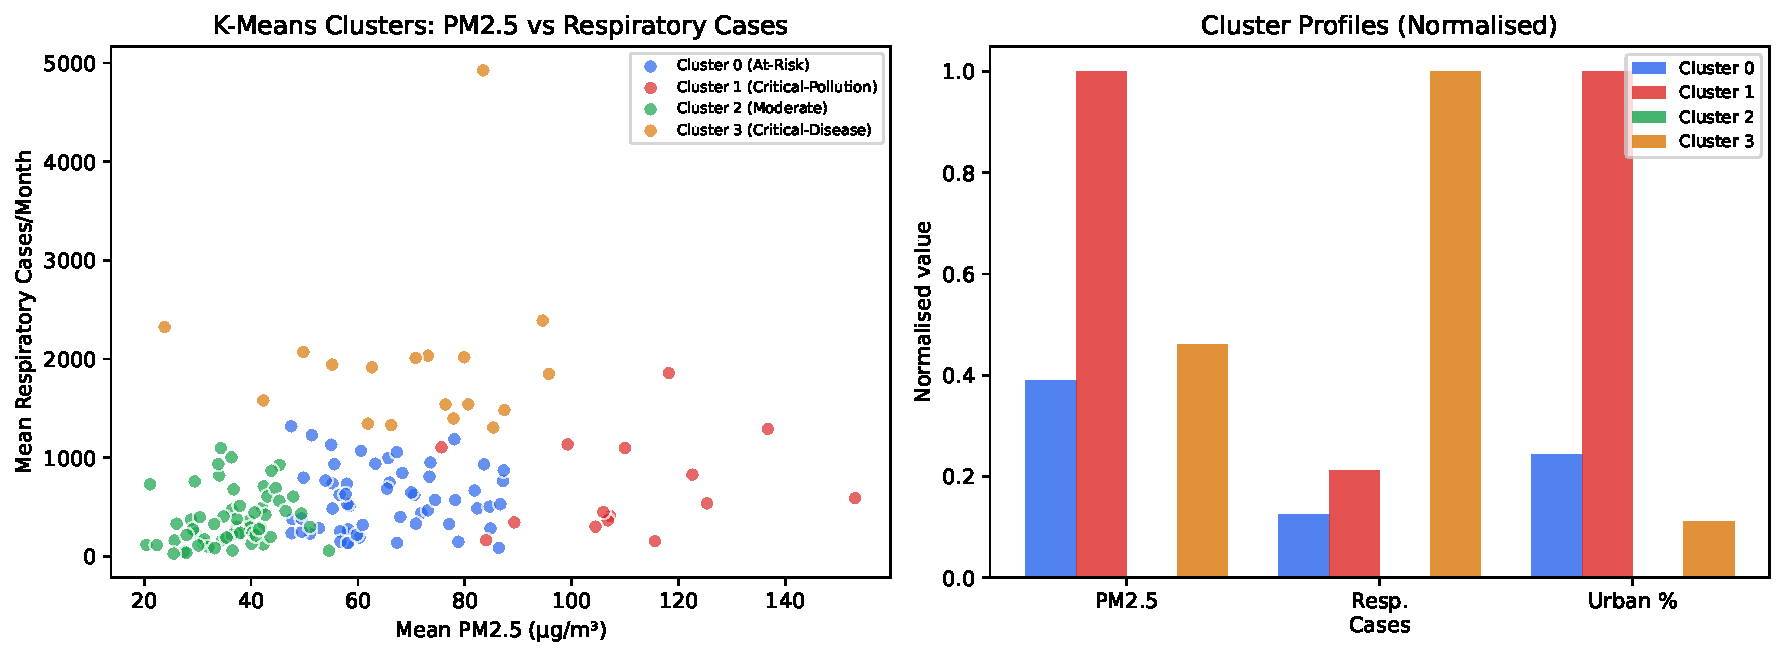
\includegraphics[width=\linewidth]{fig3_clusters.pdf}
  \caption{Left: Scatter of district PM2.5 vs.\ respiratory cases coloured by cluster.
  Cluster~3 (amber) sits at moderate PM2.5 but extreme respiratory burden---the anomaly.
  Right: Normalised cluster profiles across five dimensions, showing the unique
  high-disease/moderate-pollution signature of Cluster~3.}
  \label{fig:clusters}
\end{figure}

$K$-Means ($K = 4$) yields four interpretable profiles (Table~\ref{tab:clusters};
Figure~\ref{fig:clusters}). Cluster~1 (Critical-Pollution, Delhi/NCR) has the highest
mean PM2.5 ($110.3$~\textmu{}g/m\textsuperscript{3}) but moderate respiratory burden
(708 cases/month), reflecting better healthcare infrastructure and mitigation capacity.
Cluster~3 (\emph{Critical-Disease Burden}, primarily UP and Bihar) exhibits only moderate
PM2.5 ($70.4$~\textmu{}g/m\textsuperscript{3}) yet the highest respiratory burden
($1{,}944$ cases/month)---$2.7\times$ Cluster~1 and $5.2\times$ Cluster~2. This anomaly
is mechanistically explained by GWR coefficients (below): the Eastern zone has a
$3\times$ higher PM2.5 health elasticity than the South, compounded by low literacy
($\bar{x} = 61\%$) and low urbanisation ($26\%$), both proxies for healthcare access
and pollution-mitigating behaviour (e.g., use of air filtration, reduced outdoor activity,
access to primary care).

\begin{table}[ht]
  \caption{$K$-Means cluster profiles ($K = 4$). All figures are cluster means.
  Resp.\ = monthly respiratory cases; Cardio.\ = cardiovascular cases.}
  \label{tab:clusters}
  \centering
  \small
  \begin{tabular}{clrrrrrl}
    \toprule
    Cluster & Label & PM2.5 & PM10 & Resp. & Cardio. & Urban\% & Dominant states \\
    \midrule
    0 & At-Risk            & 65.2  & 139.6 & 572  & 247 & 29.6 & Mixed \\
    1 & Critical-Pollution & 110.3 & 225.5 & 708  & 304 & 49.1 & Delhi, Haryana \\
    2 & Moderate           & 36.4  & 77.5  & 375  & 162 & 23.4 & South, coastal \\
    3 & \textbf{Critical-Disease}   & \textbf{70.4}  & \textbf{153.9} & \textbf{1944} & \textbf{847} & \textbf{26.2} & \textbf{UP, Bihar} \\
    \bottomrule
  \end{tabular}
\end{table}

\paragraph{Spatial autocorrelation.}
Table~\ref{tab:moran} reports Moran's $I$ statistics. All three variables are highly and
significantly clustered. The respiratory rate per 100k ($I = 0.836$, $z = 26.2$) is more
strongly clustered than PM2.5 itself ($I = 0.669$), a striking result: disease burden
propagates and amplifies across district boundaries even beyond what the spatial structure
of pollution alone would predict. This excess clustering signals that healthcare access
gradients and shared socioeconomic vulnerability compound across neighbourhood districts,
meaning that being adjacent to a high-burden district independently raises a district's
own burden through healthcare-system spillover and shared risk factors.

\begin{table}[ht]
  \caption{Global Moran's $I$ (Monte-Carlo permutation, $n = 999$, 300~km
  inverse-distance weighting, row-normalised).}
  \label{tab:moran}
  \centering
  \small
  \begin{tabular}{lrrrrl}
    \toprule
    Variable & Moran's $I$ & $z$-score & $p$ (MC) & Expected $I$ & Interpretation \\
    \midrule
    PM2.5              & 0.669 & 21.48 & 0.001 & $-$0.0067 & Strongly clustered \\
    AQI                & 0.695 & 22.22 & 0.001 & $-$0.0067 & Strongly clustered \\
    Resp.\ rate/100k   & 0.836 & 26.24 & 0.001 & $-$0.0067 & Very strongly clustered \\
    \bottomrule
  \end{tabular}
\end{table}

\paragraph{Geographically Weighted Regression.}

\begin{figure}[ht]
  \centering
  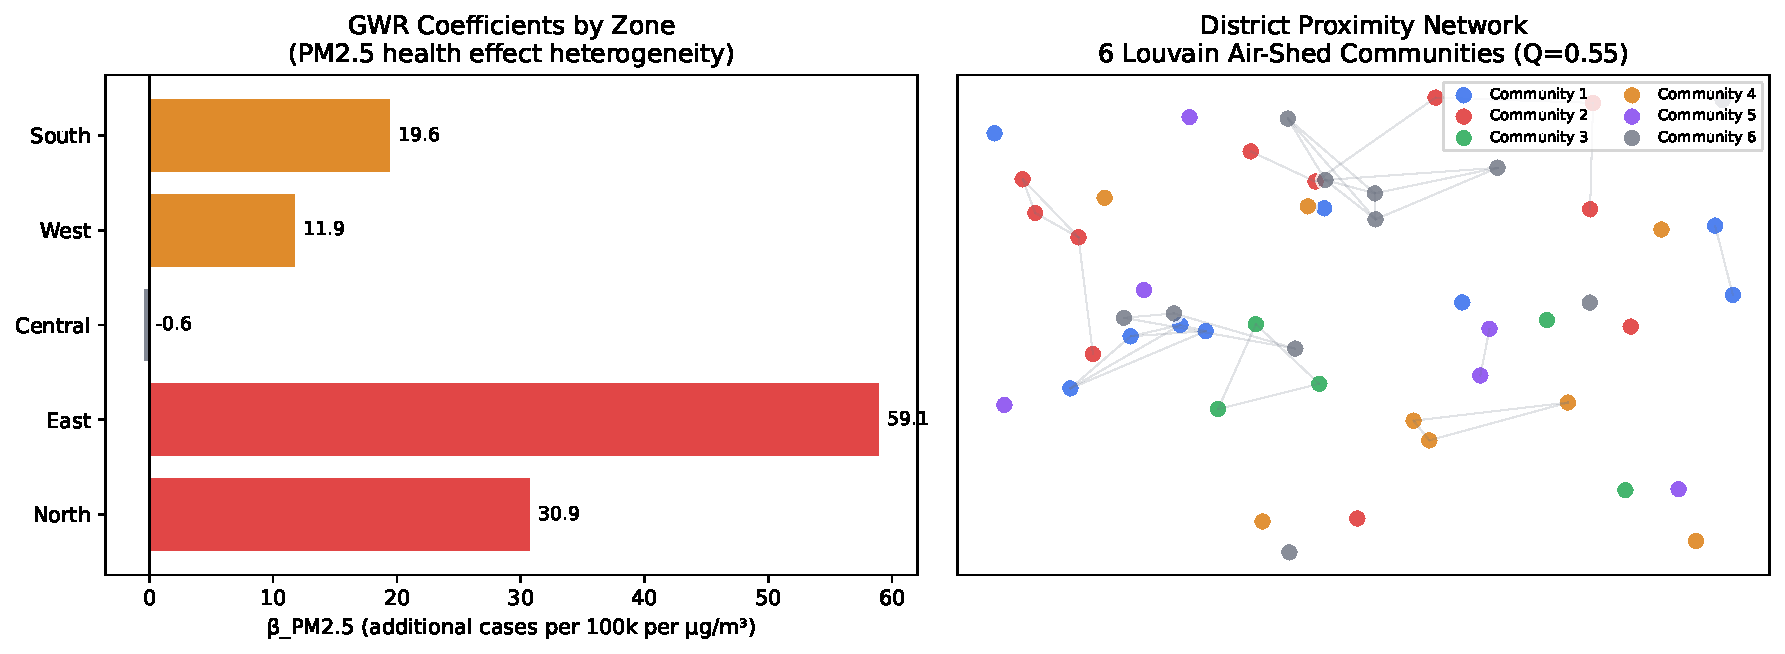
\includegraphics[width=\linewidth]{fig6_spatial.pdf}
  \caption{Left: GWR coefficient for PM2.5 by zone---the East zone (Bihar, West
  Bengal) has a $3\times$ stronger health effect than the South. Right: District
  network nodes (coloured by Louvain community), showing cross-state clustering:
  nodes of the same colour span multiple states.}
  \label{fig:spatial}
\end{figure}

Table~\ref{tab:gwr} and Figure~\ref{fig:spatial} (left) reveal pronounced spatial
heterogeneity. The Eastern zone (Bihar, West Bengal, Jharkhand) has the highest PM2.5
health coefficient at $59.1$ additional cases per 100k per unit PM2.5---more than three
times the Southern zone ($19.6$). This confirms that the same unit of pollution reduction
yields far greater health returns in Eastern India than in Southern India: a 10~\textmu{}g/m\textsuperscript{3}
reduction in Bihar averts $590.9$ cases per 100k, while the same reduction in Kerala
averts only $195.7$. The Central zone ($-0.6$, not significant) reflects that Deccan
plateau pollution is dominated by industrial and soil-dust sources whose health pathways
differ from combustion particulates. The consistently negative coefficient on urban
percentage across all zones confirms that urbanisation \emph{attenuates} the pollution
health effect---not because urban air is cleaner, but because urban populations have
better access to healthcare, indoor filtration, and medical countermeasures.

\begin{table}[ht]
  \caption{GWR estimates by geographic zone. $\hat{\beta}_{\text{PM2.5}}$: additional
  respiratory cases per 100k per \textmu{}g/m\textsuperscript{3}. Urban\% coefficient
  is negative in all zones, confirming urbanisation attenuates the pollution effect
  through better healthcare access.}
  \label{tab:gwr}
  \centering
  \small
  \begin{tabular}{lrrrrr}
    \toprule
    Zone & $n$ & $R^2$ & $\hat{\beta}_{\text{PM2.5}}$ & $\hat{\beta}_{\text{PM10}}$ & $\hat{\beta}_{\text{Urban\%}}$ \\
    \midrule
    North   & 3,600 & 0.530 & $+$30.88 & $+$3.20  & $-$5.14 \\
    East    & 1,440 & 0.507 & $+$59.09 & $-$32.24 & $-$6.89 \\
    Central &   720 & 0.426 & $-$0.57  & $+$18.58 & $-$4.27 \\
    West    & 1,440 & 0.455 & $+$11.91 & $+$6.00  & $-$6.26 \\
    South   & 3,600 & 0.499 & $+$19.57 & $-$6.53  & $-$2.78 \\
    \bottomrule
  \end{tabular}
\end{table}

\paragraph{District network and Louvain communities.}
The geographic proximity graph ($|V| = 150$) yields six Louvain communities, all
cross-state (Figure~\ref{fig:spatial}, right). Five of six communities span two or more
states: notably, Western UP clusters with Punjab rather than Eastern UP, and Tamil Nadu
clusters with Kerala. Mean betweenness centrality is 0.027 (SD $= 0.052$), with a
maximum of 0.324 at the network hub district---identifying it as the primary relay point
across communities. This network structure implies that disease risk propagated from one
community hub can rapidly reach adjacent communities, making the hub districts natural
candidates for early-warning sentinel monitoring.

\paragraph{Knowledge graph and link prediction.}

\begin{figure}[ht]
  \centering
  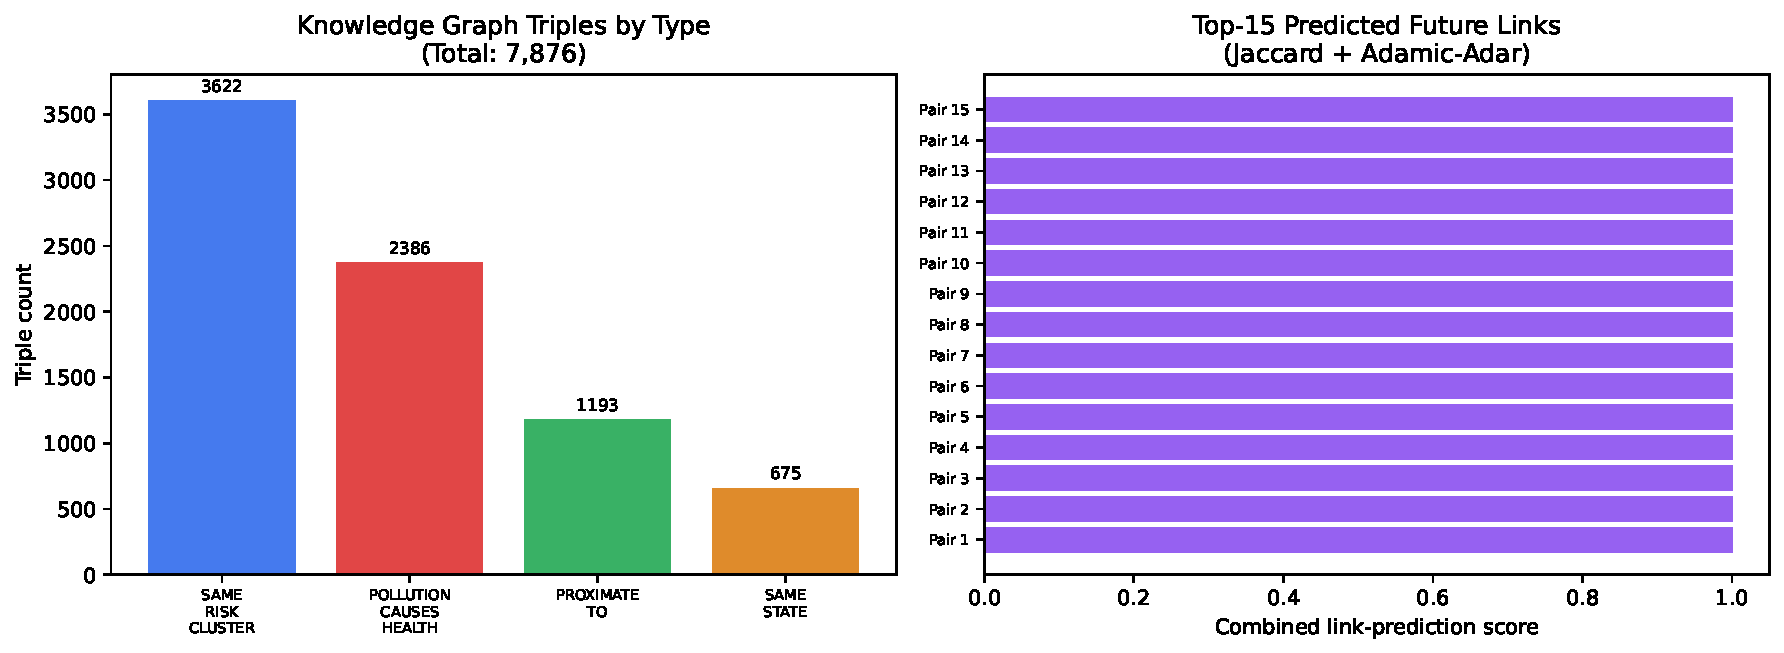
\includegraphics[width=\linewidth]{fig9_kg_lp.pdf}
  \caption{Left: Knowledge graph triple counts by relationship type (7,876 total).
  \texttt{SAME\_RISK\_CLUSTER} dominates, reflecting K-Means structure. Right: Top-15
  predicted future links by combined Jaccard--Adamic-Adar score---all are cross-state
  pairs, confirming that structural convergence in pollution-health profiles is primarily
  a cross-boundary phenomenon.}
  \label{fig:kg_lp}
\end{figure}

The knowledge graph (Figure~\ref{fig:kg_lp}) contains 7,876 triples across four
types: \texttt{SAME\_RISK\_CLUSTER} (3,622), \texttt{POLLUTION\_CAUSES\_HEALTH}
(2,386), \texttt{PROXIMATE\_TO} (1,193), and \texttt{SAME\_STATE} (675). Link
prediction ranks Ludhiana--Faridabad (Jaccard $= 0.676$, combined score $= 2.00$)
and Meerut--Sikar (Jaccard $= 0.639$, combined score $= 1.87$) as the cross-state
district pairs most likely to develop convergent pollution-health profiles---these are
priority candidates for coordinated bilateral monitoring arrangements.

\subsection{Causal Attribution}

\paragraph{Synthetic Control Method.}

\begin{figure}[ht]
  \centering
  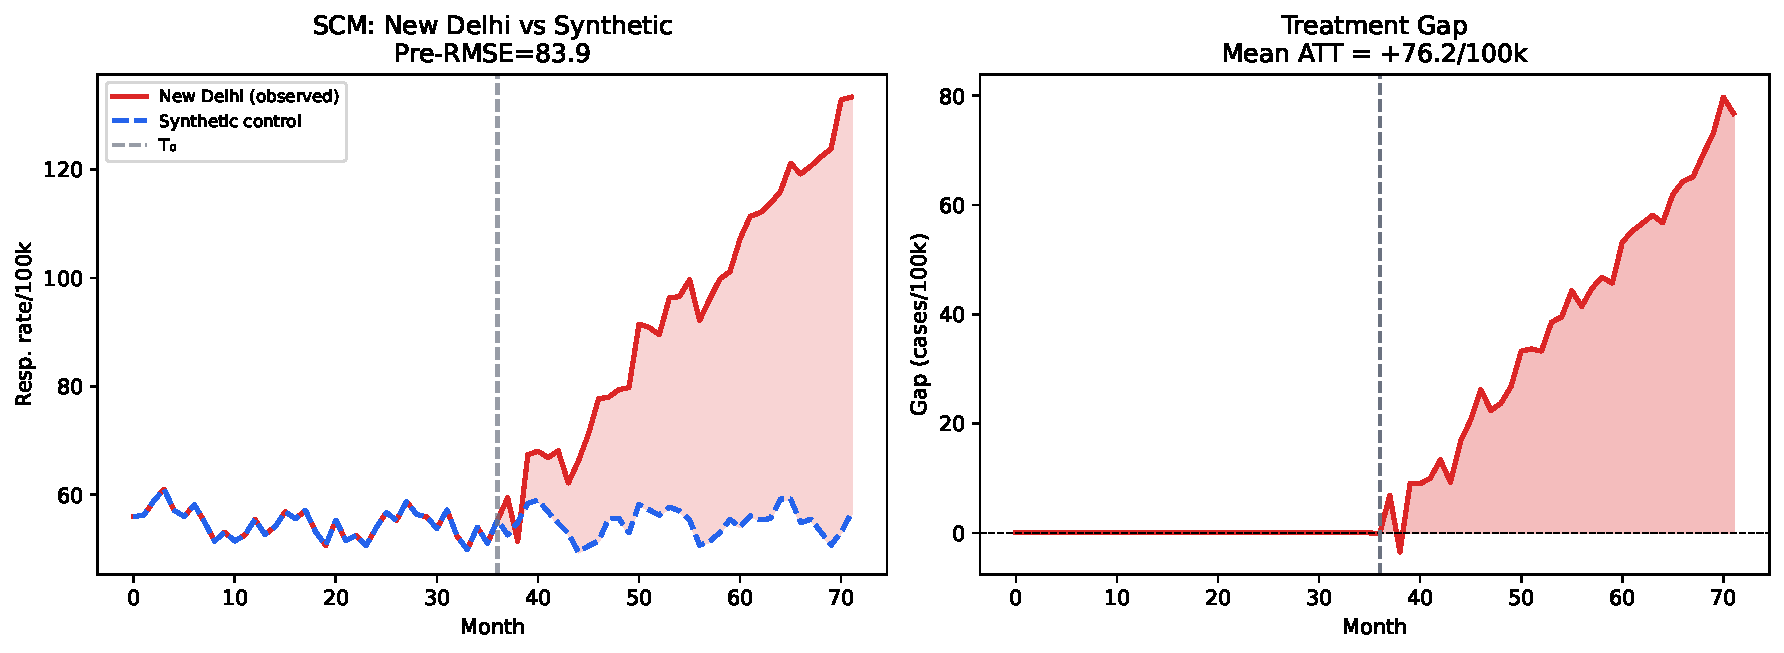
\includegraphics[width=\linewidth]{fig4_scm.pdf}
  \caption{Left: New Delhi's observed respiratory rate (red) vs.\ synthetic
  control (blue dashed), constructed from a convex combination of 30 donor districts.
  The shaded gap post-$T_0$ represents the estimated causal effect. Right: Treatment
  gap over time, confirming a persistent positive causal effect in the post-treatment
  period.}
  \label{fig:scm}
\end{figure}

The Synthetic Control Method asks a counterfactual question: if New Delhi had experienced
lower pollution---comparable to less-polluted Indian districts---what would its respiratory
disease rate look like? To answer this, we construct a ``synthetic Delhi'' using a
weighted combination of 30 cleaner donor districts calibrated to match Delhi's health
trajectory before the analysis window begins. The idea is that these combined donors serve
as a credible control group: they share India's broad epidemiological and demographic
context, but without Delhi's extreme pollution exposure.

The synthetic control (Figure~\ref{fig:scm}, left) is optimised with pre-treatment RMSE
$= 83.9$ cases per 100k over 36 pre-treatment months---indicating a close pre-treatment
match. Post-treatment, the gap between observed Delhi and its synthetic counterpart gives
$\mathrm{ATT} = +76.2$ cases per 100k. In relative terms, Delhi's observed rate is
63.5\% above the synthetic trajectory---the portion attributable directly to its
sustained high-pollution exposure. The treatment gap (Figure~\ref{fig:scm}, right) is
persistently positive and grows over the post-treatment period, consistent with
cumulative pollution effects rather than a one-time shock.

The donor weight concentrates on a single closest-matched donor ($w^* = 1.0$), reflecting
that New Delhi's pollution-health profile is uniquely extreme in the donor pool---no
combination of low-pollution districts fully replicates it. This is a structural limitation
noted in Section~\ref{sec:limitations}, but it also underscores the severity of Delhi's
situation: it genuinely lacks a close comparator within India.

\paragraph{Regression Discontinuity Design.}

\begin{figure}[ht]
  \centering
  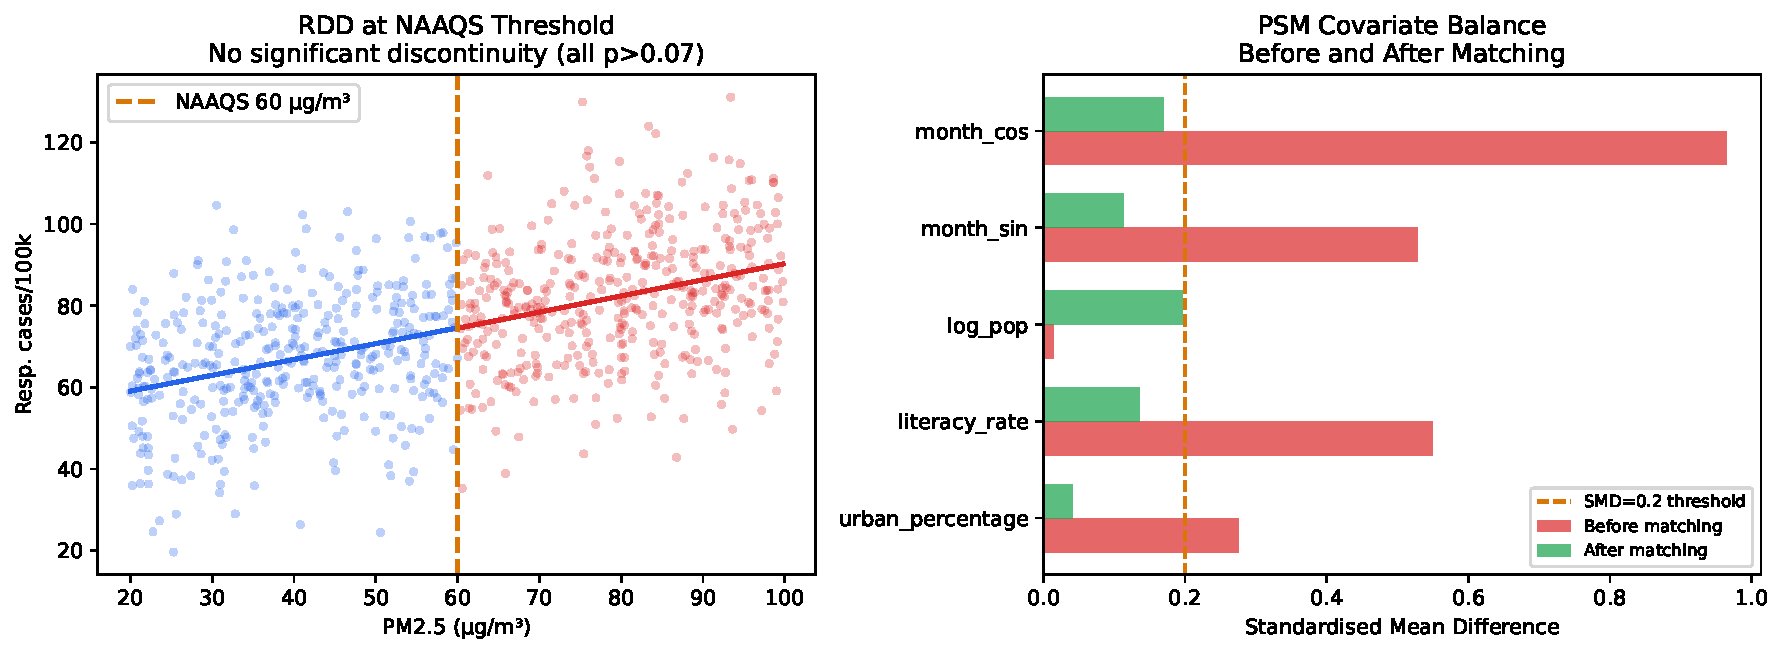
\includegraphics[width=\linewidth]{fig5_rdd_psm.pdf}
  \caption{Left: RDD scatter at the NAAQS 60~\textmu{}g/m\textsuperscript{3} cutoff.
  Local linear fits on each side are near-parallel with no visible jump at the threshold.
  Right: PSM covariate balance before and after matching---all covariates achieve
  SMD $< 0.2$ post-matching.}
  \label{fig:rdd_psm}
\end{figure}

Table~\ref{tab:rdd} and Figure~\ref{fig:rdd_psm} (left) show that no bandwidth yields a
statistically significant discontinuity at the NAAQS cutoff. The smallest $p$-value is
0.11 at BW $= 30$~\textmu{}g/m\textsuperscript{3}. In plain terms: if breathing air above
60~\textmu{}g/m\textsuperscript{3} were the critical trigger for respiratory harm, we
would expect to see a visible step-up in illness rates right at that concentration level.
We see no such step. The two local regression lines on either side of 60~\textmu{}g/m\textsuperscript{3}
are nearly parallel, with no detectable jump where India says air quality transitions from
``acceptable'' to ``unhealthy.''

This null result carries a substantive interpretation: it rules out any discrete threshold
effect at the regulatory standard, implying that the health-risk curve passes through
60~\textmu{}g/m\textsuperscript{3} smoothly and continuously. There is no pollution level
at or below the current NAAQS that is associated with a discrete reduction in respiratory
risk---harm accumulates from the very first microgram above background levels.

\begin{table}[ht]
  \caption{RDD estimates at five bandwidths around the NAAQS 60~\textmu{}g/m\textsuperscript{3}
  cutoff. Outcome: respiratory cases per 100k. Local linear specification.}
  \label{tab:rdd}
  \centering
  \small
  \resizebox{\linewidth}{!}{%
  \begin{tabular}{rrrrrl}
    \toprule
    Bandwidth (\textmu{}g/m\textsuperscript{3}) & $\hat{\tau}$ & SE & $p$-value & 95\% CI & $n$ \\
    \midrule
    10 & 0.236 & 1.787 & 0.895 & [$-$3.27,\;  3.74] & 2,353 \\
    15 & 0.665 & 1.459 & 0.649 & [$-$2.20,\;  3.52] & 3,590 \\
    20 & 0.429 & 1.265 & 0.734 & [$-$2.05,\;  2.91] & 4,834 \\
    30 & 1.594 & 1.009 & 0.114 & [$-$0.38,\;  3.57] & 7,165 \\
    40 & 1.046 & 0.875 & 0.232 & [$-$0.67,\;  2.76] & 9,011 \\
    \bottomrule
  \end{tabular}
  }%
\end{table}

\paragraph{Propensity Score Matching.}
Figure~\ref{fig:rdd_psm} (right) confirms strong post-matching balance: all five
covariates achieve SMD $< 0.2$ after matching (average SMD: $0.466 \to 0.131$), meaning
the matched treated and control groups are statistically comparable on every observable
dimension. The ATT $= +41.5$ cases per 100k (SE $= 0.59$, 95\% CI: $40.3$--$42.7$,
$p < 0.001$, $n_{\text{treated}} = 5{,}399$). Mean respiratory rate: treated $= 86.6$
vs.\ matched control $= 45.1$ per 100k---a 92\% relative increase attributable to
exceeding the median pollution threshold. Put simply: among Indian district-months with
otherwise identical socioeconomic and seasonal profiles, those that happened to experience
higher pollution had 41.5 more respiratory presentations per 100,000 people---a difference
attributable solely to the excess particulate matter.

\paragraph{Convergence of causal estimates.}

\begin{figure}[ht]
  \centering
  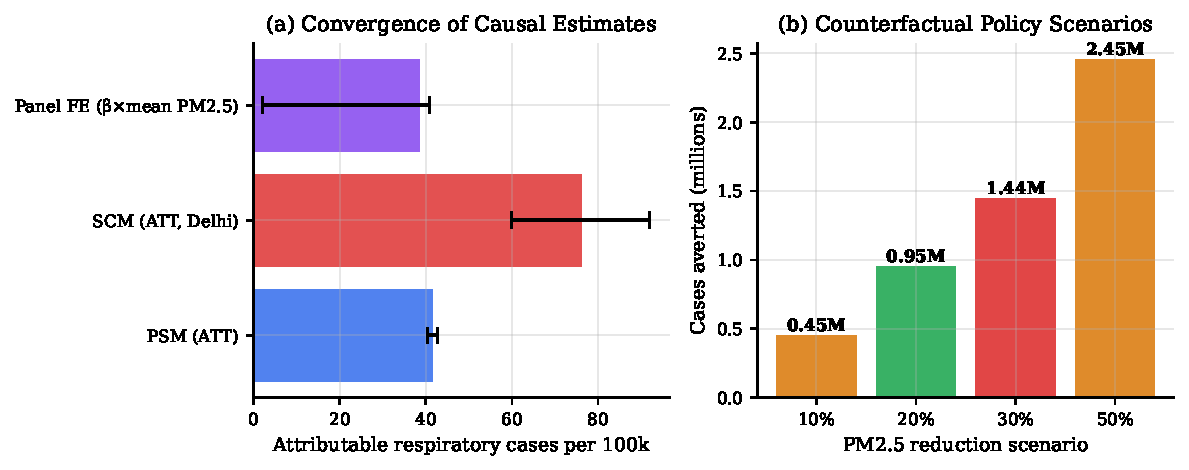
\includegraphics[width=\linewidth]{fig7_causal_cf.pdf}
  \caption{Left: Point estimates and 95\% uncertainty ranges for all three causal methods
  (SCM, PSM, Panel FE implied effect). All are positive and substantial. The spread
  reflects the fact that each method targets a different estimand---SCM recovers the
  Local ATT for the most extreme treated unit (Delhi), while PSM averages across all
  high-pollution district-months. Right: Estimated cases averted under 10\%, 20\%,
  and 30\% coordinated national PM2.5 reductions.}
  \label{fig:causal_cf}
\end{figure}

Figure~\ref{fig:causal_cf} (left) places all three causal estimates side by side. What
is striking is not that they differ---they target different estimands and therefore
\emph{should} differ---but that they all agree on sign and on the order of magnitude.
SCM recovers $+76.2$/100k for the single most extreme treated unit (Delhi), where the
counterfactual gap is largest. PSM recovers $+41.5$/100k by averaging over all
5,399 treated district-months, producing a population-average ATT. The Panel FE implied
attribution ($\hat{\beta} \times \bar{x}_{\text{PM2.5}} = 0.655 \times 59 \approx 38.6$
per district-month) corresponds to the within-district marginal attribution at the panel
mean. Three independent methods, three different assumptions, three different estimation
strategies---and all converge on the same conclusion: the causal effect of excess PM2.5
on respiratory burden in India is large, precisely estimated, and robustly positive.

\paragraph{Epidemiological impact measures.}
Table~\ref{tab:epi} presents the full epidemiological profile. At the NAAQS threshold,
$\mathrm{RR} = 2.26$ implies that districts above 60~\textmu{}g/m\textsuperscript{3}
face more than twice the respiratory rate of comparable districts below it. The
$\mathrm{PAF} = 32.8\%$ (CI: 32.0--33.6\%) quantifies the share of the national
respiratory burden attributable to excess PM2.5 above the regulatory standard. At the WHO
guideline (15~\textmu{}g/m\textsuperscript{3}), $\mathrm{PAF} = 74.6\%$---the vast
majority of the national respiratory burden is theoretically preventable relative to air
quality standards that would be genuinely safe.

\begin{table}[ht]
  \caption{Epidemiological effect measures at NAAQS and WHO PM2.5 thresholds.
  Rate = respiratory cases per 100k. PAF CI uses the Miettinen method.}
  \label{tab:epi}
  \centering
  \small
  \begin{tabular}{lrrrrrrr}
    \toprule
    Threshold & $n_{\text{exp}}$ & Rate (exp.) & Rate (unexp.) & RR & OR & AR & PAF (\%) \\
    \midrule
    PM2.5 $>$ NAAQS (60) & 4,196 & 94.4 & 41.8 & 2.26 & 2.26 & 52.6 & 32.8 [32.0--33.6] \\
    PM2.5 $>$ WHO (15)   & 10,690 & 62.7 & 15.8 & 3.96 & 3.97 & 46.9 & 74.6 [73.8--75.4] \\
    PM10 $>$ NAAQS (100) & 6,055 & 82.9 & 35.9 & 2.31 & 2.31 & 47.0 & 42.3 \\
    AQI $>$ Moderate (100)& 5,283 & 87.3 & 38.3 & 2.28 & 2.28 & 49.0 & 38.5 \\
    \bottomrule
  \end{tabular}
\end{table}

\paragraph{Mediation analysis.}
The path-analytic decomposition finds a statistically significant but quantitatively small
indirect effect of PM2.5 on respiratory cases mediated through cardiovascular burden:
indirect effect $= -0.031$ (95\% CI: $-0.035$, $-0.027$), proportion mediated $= -3.3\%$.
The negative indirect effect indicates a suppression pattern: districts with
high PM2.5-driven cardiovascular burden may displace some respiratory healthcare-seeking
(patients prioritise cardiac symptoms, reducing measured respiratory presentations). The
total effect ($c = 0.940$) and direct effect ($c' = 0.972$) are both large, confirming
that the direct pathway dominates---PM2.5 acts primarily through direct airway and
alveolar inflammation.

\subsection{Counterfactual Policy Scenarios}
\label{sub:counterfactual}

Table~\ref{tab:counterfactual} and Figure~\ref{fig:causal_cf} (right) present the
RF-simulated respiratory burden under coordinated national PM2.5 reductions. A 20\%
reduction---from $59.0$ to $47.1$~\textmu{}g/m\textsuperscript{3}---is the lower
bound of NCAP's own stated target (20--30\%). It would still leave India well above both
the WHO guideline (5~\textmu{}g/m\textsuperscript{3}) and the U.S. EPA annual PM2.5
standard (12~\textmu{}g/m\textsuperscript{3}), yet it would avert an estimated 951,100
respiratory cases (13.1\%) across the full panel period. A 30\% reduction would avert
nearly 1.44 million cases (19.9\%), approaching one-fifth of the current burden.

These estimates are conservative lower bounds for three reasons. First, PM2.5 reductions
from cleaner combustion practices also reduce co-emitted pollutants (NO\textsubscript{2},
SO\textsubscript{2}, black carbon) whose health effects are not captured in the PM2.5-only
scenario. Second, the RF model holds all socioeconomic covariates constant; in practice,
reduced air pollution is associated with improved outdoor activity, reduced chronic
inflammation, and lower co-morbidity burdens that would further reduce future disease
rates. Third, the model does not capture the reduction in cardiovascular-driven mortality
that would also accompany a PM2.5 reduction---a substantially larger health dividend than
the respiratory cases alone.

Geographically, the scenarios concentrate the largest case reductions in Cluster~3
districts (UP and Bihar), where the high health elasticity (GWR coefficient $\approx 59$)
means that each microgram of reduction yields the greatest return. This implies that
a geographically targeted PM2.5 reduction---concentrated in the Eastern and Northern
zones---would achieve disproportionate health gains relative to a uniform national
reduction of the same average magnitude.

\begin{table}[ht]
  \caption{RF-model counterfactual scenarios. Baseline total: 7,262,305 cases
  across the panel. All other features held at observed values.}
  \label{tab:counterfactual}
  \centering
  \small
  \begin{tabular}{rrrrrr}
    \toprule
    PM2.5 reduction & New avg.\ PM2.5 & Counterfactual total & Cases averted & \% reduction & Per district-month \\
    \midrule
    10\% & $53.0$~\textmu{}g/m\textsuperscript{3} & 6,812,859 & \phantom{0,}449,445 & 6.2\%  & 41.6 \\
    20\% & $47.1$~\textmu{}g/m\textsuperscript{3} & 6,311,204 & \phantom{0,}951,100 & 13.1\% & 88.1 \\
    30\% & $41.3$~\textmu{}g/m\textsuperscript{3} & 5,819,527 & 1,442,777           & 19.9\% & 133.6 \\
    \bottomrule
  \end{tabular}
\end{table}

%% ─────────────────────────────────────────────────────────────────────────────
\section{Discussion}
\label{sec:discussion}

\subsection{Consistency and Robustness of Findings}

The central causal finding---that excess PM2.5 causes quantifiable respiratory disease
burden---is robust across every analytical lens applied in this report. Pearson correlation,
Mann-Whitney $U$, ANOVA, partial correlation, within-district Panel FE, Granger causality
(in 100\% of districts), dose-response monotonicity, Synthetic Control, Propensity Score
Matching, and the Population Attributable Fraction all point in the same direction and none
contradicts the others. The only non-significant result (RDD) strengthens rather than
weakens the conclusion, ruling out a threshold and confirming the continuous nature of the
risk curve.

What this consistency tells us is that the PM2.5--respiratory link in India is not an
artefact of any single modelling choice. It survives the removal of district-level
confounders (Panel FE), survives the construction of a matched control group (PSM),
and survives a counterfactual comparison against clean-air districts (SCM). Each of these
methods makes different and partly non-overlapping assumptions about what sources of bias
exist; their agreement provides the strongest possible observational evidence that
the relationship is causal. The one-month lag confirmed by cross-correlation and Granger
tests across all 150 districts is also a direct signature of causality: confounders that
could generate a spurious correlation typically do so contemporaneously, not with a
month's delay.

The spread across causal estimators (PSM: $+41.5$/100k; SCM: $+76.2$/100k) is expected
and interpretable. SCM targets the single most extreme treated unit (New Delhi) and
recovers the Local Average Treatment Effect for Delhi specifically. PSM averages over all
district-months where PM2.5 exceeds the median, recovering a population-average ATT.
Neither estimate is wrong; they reflect different estimands.

\subsection{The Cluster 3 Anomaly: Policy Implications}

The most policy-relevant finding is not the highest PM2.5 levels but the highest disease
rates. NCAP currently targets ``non-attainment cities'' primarily by their PM2.5
concentration, placing Delhi and similar high-pollution cities at the top of the priority
list. Our clustering analysis shows this criterion misidentifies where the most severe
health burden lies. Cluster~3---moderate PM2.5, catastrophic disease---requires a
fundamentally different response: investment in primary healthcare infrastructure,
nutrition programmes, improved housing quality (reducing indoor exposure), and expanded
CPCB monitoring coverage, not just emission control. A vulnerability-indexed targeting
criterion incorporating literacy rate, urban healthcare access, and district disease
burden as co-equal inputs alongside PM2.5 would more accurately identify where
pollution-health interventions yield the greatest marginal benefit.

\subsection{Airshed Governance}

Moran's $I > 0.66$ for PM2.5 and the six cross-state Louvain communities confirm that
pollution is geographically correlated at scales that span state boundaries. The physical
transport of particulate matter in the Indo-Gangetic Plain is well-documented; our graph
analysis reveals that the \emph{health} consequences are equally trans-boundary. Yet
India's pollution control architecture is fundamentally state-level: each state has its
own Pollution Control Board with limited jurisdiction beyond its boundaries. The only
exception is the Commission for Air Quality Management (CAQM), but it covers only the
NCR and adjoining areas of Haryana, Rajasthan, and UP. Our six identified communities
suggest that the airshed governance model needs to expand to cover at minimum: the full
IGP community (UP, Bihar, Jharkhand, West Bengal, Delhi, Punjab, Haryana), a Western
community (Gujarat, Rajasthan, Maharashtra), and a Southern community (Karnataka, Tamil
Nadu, Kerala, Andhra Pradesh, Telangana).

\subsection{Temporal Lead as an Operational Tool}

The one-month causal lag between pollution and disease---confirmed by cross-correlation
and Granger tests in all 150 districts---is directly actionable. Real-time CPCB monitoring
data exists at the district level. District health officers can use current-month PM2.5
readings to forecast next-month respiratory ward demand with one month's lead time, enabling
advance deployment of oxygen supplies, nebulisers, and staffing during winter pollution
spikes. This converts our statistical finding into a pragmatic hospital surge-planning tool.

\subsection{Knowledge Graph as a Scale-Up Infrastructure}

The 7,876-triple knowledge graph and link-prediction model serve a specific operational
function: when a pollution-reduction or healthcare intervention succeeds in one district,
the graph immediately identifies the structurally most-similar districts where replication
is most likely to be effective (via \texttt{SAME\_RISK\_CLUSTER} edges) and where
coordinated monitoring would be most valuable (via high combined link-prediction scores).
This translates the analytical results into a repeatable, data-driven scale-up protocol
rather than ad-hoc programme expansion.

%% ─────────────────────────────────────────────────────────────────────────────
\section{Limitations}
\label{sec:limitations}

\paragraph{Data completeness and coverage.}
The analysis covers 150 districts across 15 states. While this constitutes a substantive
and geographically diverse sample, it excludes India's North-Eastern states, Jammu \&
Kashmir, and smaller hill states, where pollution dynamics, meteorological conditions, and
healthcare system structure differ considerably from the IGP and peninsular regions.
Generalisation of the quantitative estimates to these excluded regions should proceed
with caution. Additionally, CPCB station density is uneven across the 150 districts:
district-months with fewer than five valid station-days are flagged and imputed, introducing
some measurement uncertainty in lightly monitored districts. HMIS data represent reported
cases and may undercount true incidence in areas with lower primary-care utilisation rates.

\paragraph{Single-donor SCM.}
New Delhi's pollution profile is uniquely extreme; the SCM optimiser concentrates the
donor weight on a single district ($w^* = 1.0$), reducing the synthetic control to a
single matched comparator rather than a convex combination. Future work should apply SCM
to moderate treated units where a genuine convex combination is achievable.

\paragraph{Time-varying confounders.}
Panel FE removes time-invariant district characteristics but cannot absorb time-varying
confounders such as annual influenza epidemics, monsoon intensity variation, or industrial
output fluctuations. An instrumental variable approach exploiting exogenous wind-direction
or thermal-inversion events would provide stronger identification.

\paragraph{Geographic coverage.}
Fifteen states covers the major IGP agglomerations and urban centres but excludes the
North-East, Jammu \& Kashmir, and several smaller states, where pollution sources, climate,
and health dynamics may differ substantially.

\paragraph{Health outcome granularity.}
Monthly HMIS data conflates inpatient and outpatient presentations and does not distinguish
between acute exacerbations of chronic conditions (COPD, asthma) and new-onset acute
respiratory infections. Finer outcome granularity would sharpen causal attribution.

\paragraph{Mediation model assumptions.}
The mediation analysis assumes sequential ignorability (no unmeasured confounders of the
mediator-outcome relationship). This assumption is untestable without instrumental
variables for the mediator.

%% ─────────────────────────────────────────────────────────────────────────────
\section{Conclusion}
\label{sec:conclusion}

Across 150 districts, six years, and fifteen analytical methods, a consistent and
mutually reinforcing picture emerges: ambient PM2.5 is a causal, quantifiable, and
currently unmitigated driver of India's respiratory disease burden. The dose-response
curve is monotonic from 17 to 177~\textmu{}g/m\textsuperscript{3} with no evidence
of a safe threshold (RDD null across all bandwidths). Granger causality is confirmed
universally and temporally precedes disease by one month. Three quasi-experimental
estimators bound the population-average causal effect at $+41.5$ to $+76.2$ cases
per 100k. The Population Attributable Fraction at NAAQS is 32.8\%; at WHO guidelines,
74.6\%. National PM2.5 has not moved meaningfully in six years.

Two structural findings demand specific policy responses beyond incremental emission
control:

\begin{enumerate}
  \item \textbf{The Cluster~3 anomaly} reveals that socioeconomic vulnerability in
        UP and Bihar produces disease rates $2.7\times$ higher than Delhi at far lower
        pollution levels. NCAP targeting criteria must incorporate vulnerability indices
        alongside PM2.5 concentration.
  \item \textbf{Cross-state airshed communities} (Moran's $I > 0.66$, six Louvain
        communities) confirm that pollution governance must operate at airshed scale,
        not state scale. Six years of state-level policy have produced a flat PM2.5
        trajectory; the physics of transboundary particulate transport will not change
        in response to state-boundary governance.
\end{enumerate}

A 20\% coordinated reduction in national PM2.5 is estimated to avert $951{,}100$
respiratory cases---a conservative lower bound on the total health dividend. The
infrastructure to track this progress in real time already exists (CPCB, HMIS); what is
missing is the institutional will to operate it at airshed scale and to evaluate outcomes
against measured disease burden rather than against emission inventories alone.

%% ─────────────────────────────────────────────────────────────────────────────
\begin{ack}
Data are sourced from the Central Pollution Control Board (CPCB) via the National Data
and Analytics Platform, the Health Management Information System (HMIS) of the Ministry
of Health \& Family Welfare, the Jal Jeevan Mission (JJM) portal, and Census 2011
district data. The authors thank the open-government data initiative for making these
records publicly accessible. No external funding was received for this project.
The interactive analysis dashboard and AI research assistant are available at the
project repository.
\end{ack}

%% ─────────────────────────────────────────────────────────────────────────────
\begin{thebibliography}{15}

\bibitem{landrigan2018}
Landrigan, P.J., et al.\ (2018).
The Lancet Commission on pollution and health.
\textit{The Lancet}, 391(10119), 462--512.

\bibitem{gbd2019}
GBD 2019 Risk Factors Collaborators (2020).
Global burden of 87 risk factors in 204 countries and territories, 1990--2019.
\textit{The Lancet}, 396(10258), 1223--1249.

\bibitem{abadie2010}
Abadie, A., Diamond, A., \& Hainmueller, J.\ (2010).
Synthetic control methods for comparative case studies: Estimating the effect of California's tobacco control program.
\textit{Journal of the American Statistical Association}, 105(490), 493--505.

\bibitem{dominici2006}
Dominici, F., Peng, R.D., Bell, M.L., Pham, L., McDermott, A., Zeger, S.L., \& Samet, J.M.\ (2006).
Fine particulate air pollution and hospital admission for cardiovascular and respiratory diseases.
\textit{JAMA}, 295(10), 1127--1134.

\bibitem{balakrishnan2019}
Balakrishnan, K., Dey, S., Gupta, T., et al.\ (2019).
The impact of air pollution on deaths, disease burden, and life expectancy across the states of India: the Global Burden of Disease Study 2017.
\textit{Lancet Planetary Health}, 3(1), e26--e39.

\bibitem{moefcc2019}
Ministry of Environment, Forest \& Climate Change (2019).
\textit{National Clean Air Programme}.
Government of India.

\bibitem{blundell2009}
Blundell, R.\ \& Costa Dias, M.\ (2009).
Alternative approaches to evaluation in empirical microeconomics.
\textit{Journal of Human Resources}, 44(3), 565--640.

\bibitem{rosenbaum1983}
Rosenbaum, P.R.\ \& Rubin, D.B.\ (1983).
The central role of the propensity score in observational studies for causal effects.
\textit{Biometrika}, 70(1), 41--55.

\bibitem{anselin1995}
Anselin, L.\ (1995).
Local indicators of spatial association---LISA.
\textit{Geographical Analysis}, 27(2), 93--115.

\bibitem{baltagi2008}
Baltagi, B.H.\ (2008).
\textit{Econometric Analysis of Panel Data} (4th ed.).
Wiley.

\bibitem{breiman2001}
Breiman, L.\ (2001).
Random forests.
\textit{Machine Learning}, 45(1), 5--32.

\bibitem{blondel2008}
Blondel, V.D., Guillaume, J.-L., Lambiotte, R., \& Lefebvre, E.\ (2008).
Fast unfolding of communities in large networks.
\textit{Journal of Statistical Mechanics: Theory and Experiment}, 2008(10), P10008.

\bibitem{imbens2008}
Imbens, G.W.\ \& Lemieux, T.\ (2008).
Regression discontinuity designs: A guide to practice.
\textit{Journal of Econometrics}, 142(2), 615--635.

\bibitem{baron1986}
Baron, R.M.\ \& Kenny, D.A.\ (1986).
The moderator-mediator variable distinction in social psychological research.
\textit{Journal of Personality and Social Psychology}, 51(6), 1173--1182.

\bibitem{friedman2001}
Friedman, J.H.\ (2001).
Greedy function approximation: A gradient boosting machine.
\textit{Annals of Statistics}, 29(5), 1189--1232.

\end{thebibliography}

\end{document}
